\documentclass[10pt, a4paper, twoside=false, headsepline]{scrbook}
\usepackage[T1]{fontenc} % Umlaute
\usepackage[utf8]{inputenc} % Textcodierung
\usepackage[english]{babel} % Silbentrennung
%\usepackage{marvosym, amsmath, amssymb} % Symbole, Formeln, amssymb > mathdesign
\usepackage{lmodern, microtype} % enhanced CM, mikrotypografische Feinheiten
%\usepackage{graphicx} % Grafiken
\usepackage[hidelinks]{hyperref} % Hyperlinks
\usepackage[dvipsnames]{xcolor} % Farben (goo.gl/sP8iP, S.38)
%\usepackage[charter]{mathdesign} % Schriftart B. Charter
%\usepackage{mathptmx} % Schriftart Times
\usepackage[autolanguage]{numprint} % Zahlen

\usepackage[
  automark,
  autooneside=false
]{scrlayer-scrpage}
\clearpairofpagestyles
\ihead{\rightmark}
\ohead{\leftmark}
\ofoot[\pagemark]{\pagemark}

\usepackage{setspace}
\usepackage{anysize}
\marginsize{3cm}{3cm}{2cm}{2cm}
\setlength{\parskip}{1.3ex plus 0.2ex minus 0.2ex}
\setlength{\parindent}{0pt}

\usepackage{booktabs, tabularx} % Tabellen spacing/lines, linebreak/width
%\newcolumntype{Y}{>{\raggedright\arraybackslash}X}

\usepackage{csquotes} % Recommended addition for biblatex

\usepackage[style=numeric,backend=biber,defernumbers=true]{biblatex}
\addbibresource{thesis.bib}

\usepackage{caption}
\captionsetup{labelfont=bf,format=plain,font=small}

\usepackage[firstpage]{draftwatermark} % [final]
\SetWatermarkLightness{0.9}

\usepackage{pgf-umlsd}

\usepackage{listings}
\lstset{
	%language=, % https://en.wikibooks.org/wiki/LaTeX/Source_Code_Listings#Supported_languages
	basicstyle=\ttfamily,
	columns=flexible,
	breaklines=true,
	numbers=left,
	tabsize=4,
	% Black-white
% 	numberstyle=\scriptsize,
% 	stringstyle=\color{darkgray},
% 	commentstyle=\color{gray},
% 	frame=single,
	% Colour
	numberstyle=\scriptsize\color{gray},
	stringstyle=\color{orange},
	commentstyle=\color{teal},
	keywordstyle=\bfseries\color{Blue},
	backgroundcolor=\color{black!02},
	% Special
	breakindent=0cm,
  moredelim=[is][\bfseries\color{Red}]{@}{@},
}

\let\origunderscore\_
\renewcommand{\_}{\origunderscore\allowbreak}
\newcommand{\config}[1]{\texttt{config.\allowbreak #1}}
\newcommand{\range}{from August 30 18:40 to September 1 5:10 UTC, 2015}

\begin{document}
\pagestyle{empty}
\pagenumbering{alph}
\begin{titlepage}
\titlehead{
  \begin{tabularx}{\textwidth}{lXr}
  \parbox{2.5cm}{
\includegraphics[width=2.5cm]{fau-logo}} &
  \parbox{8.5cm}{\centering
  Lehrstuhl für Informatik 1 \\
  Friedrich-Alexander-Universität \\
  Erlangen-Nürnberg} &
  \parbox{2.5cm}{
\includegraphics[width=2.5cm]{i1-logo}}
  \end{tabularx}
}
\subject{Bachelor Thesis}
\title{Analysis of BitTorrent Trackers and Peers}
\subtitle{Counting Confirmed Downloads in BitTorrent}
\author{Stefan Schindler}
\date{Erlangen, \today}
\publishers{
  \begin{tabular}{rl}
  Examiner: & Prof. Dr.-Ing. Felix Freiling \\
  Advisor: & Philipp Klein, M.\,Sc. \\
  & Michael Gruhn, M.\,Sc. \\
  & Dr. Werner Massonne
  \end{tabular}
}

\maketitle
\end{titlepage}
%%%%%%%%%%%%%%%%%%%%%%%%%%%%%%%%%%%%%%%%%%%%%%%%%%%%%%%%%%%%%%%%%%%%%%%%%%%%%%%%%

\vspace*{\fill}
\noindent
\raisebox{-0.07cm}{
\includegraphics[width=2.3cm]{by-sa}}\quad Copyright © 2015 Stefan Schindler
\medskip

\noindent
This work is licensed under the Creative Commons Attribution-ShareAlike 4.0 International License.\\
To view a copy of this license, visit \url{http://creativecommons.org/licenses/by-sa/4.0/}.
\cleardoublepage
%%%%%%%%%%%%%%%%%%%%%%%%%%%%%%%%%%%%%%%%%%%%%%%%%%%%%%%%%%%%%%%%%%%%%%%%%%%%%%%%%

\pagestyle{scrplain}
\pagenumbering{roman}
\vspace*{\fill}
\section*{Eidesstattliche Erklärung / Statutory Declaration}

\vspace{0.1cm}
\noindent\hrule
\begin{quote}
Hiermit versichere ich eidesstattlich, dass die vorliegende Arbeit von mir
selbständig, ohne Hilfe Dritter und ausschließlich unter Verwendung der
angegebenen Quellen angefertigt wurde. Alle Stellen, die wörtlich oder
sinngemäß aus den Quellen entnommen sind, habe ich als solche kennt\-lich
gemacht. Die Arbeit wurde bisher in gleicher oder ähnlicher Form keiner anderen
Prüfungsbehörde vorgelegt.
\end{quote}

\begin{quote}
I hereby declare formally that I have developed and written the enclosed thesis
entirely by myself and have not used sources or means without declaration in
the text. Any thoughts or quotations which were inferred from the sources are
marked as such. This thesis was not submitted in the same or a substantially
similar version to any other authority to achieve an academic grading.
\end{quote}
\noindent\hrule

\vspace{0.5cm}
\noindent
Der Friedrich-Alexander-Universität, vertreten durch den Lehrstuhl
für Informatik 1, wird für Zwecke der Forschung und Lehre ein
einfaches, kostenloses, zeitlich und örtlich unbeschränktes
Nutzungsrecht an den Arbeitsergebnissen der Arbeit einschließlich
etwaiger Schutz- und Urheberrechte eingeräumt.

\vspace{0.5cm}
\noindent
Erlangen, \today

\vspace{1cm}
\begin{flushright}
Stefan Schindler \quad\null
\end{flushright}
\cleardoublepage
%%%%%%%%%%%%%%%%%%%%%%%%%%%%%%%%%%%%%%%%%%%%%%%%%%%%%%%%%%%%%%%%%%%%%%%%%%%%%%%%%

\vspace*{\fill}
\begin{center}
{\large\textbf{Abstract}}
\end{center}

\begin{quote}
% Motivation
BitTorrent is the most used technology for file sharing to date and discussed to damage the creative industry. However, due to its distributed structure the extent of downloaded copies can only be estimated.
% Problem statement
The common method is to collect all IP addresses of a torrent swarm by issuing scrape and announce requests to tracker servers. After testing their reachability, this number is used as an estimation of downloads, but falsely includes peers who did not finish the download.
% Approach
This thesis will extend this method by contacting each peer continuously and learning the download progress through the BitTorrent protocol. A tool was written to do this after collecting addresses from trackers and the DHT network, and accepting incoming connections. A confirmed download was registered when a peer crossed the threshold of \numprint[\%]{98}.
% Results
For small and large torrents respectively, between \numprint[\%]{9} and \numprint[\%]{55} of the downloads reported by the main trackers in scrape responses could be confirmed over 34 hours and 19 torrents. For less than \numprint[\%]{2} of unique peer addresses a download was confirmed.
% Conclusions
Often subsequent progress evaluations of peers failed, which lowers this numbers significantly. Further adjustments to the used implementation are necessary to obtain better results.
\end{quote}

\vspace*{\fill}
\begin{center}
{\large\textbf{Zusammenfassung}}
\end{center}

\begin{quote}
% Motivation
BitTorrent ist die meistgenutzte Filesharing-Technologie, wobei die Schädlichkeit für die Kreativindustrie diskutiert wird. Jedoch kann man den Umfang an heruntergeladenen Kopien nur abschätzen.
% Problem statement
Üblicherweise werden dafür alle IP-Adressen eines Torrent-Schwarms mithilfe von Scrape- und Announce-Anfragen an die Tracker-Server gesammelt. Nachdem deren Erreichbarkeit getestet wurde, wird diese Zahl als Abschätzung der Downloads genutzt, wobei Peers, die den Download nicht abgeschlossen haben, fälschlicherweise mitgezählt werden.
% Approach
Diese Arbeit wird diese Methode erweitern, indem jeder Peer wiederholt kontaktiert und der Download-Fortschritt mit Hilfe des BitTorrent-Protokolls extrahiert wird. Es wurde ein Programm geschrieben, das dies tut, nachdem es Adressen von Trackern und dem DHT-Netzwerk sammelt, und eingehende Verbindungen annimmt. Ein bestätigter Download wurde registriert, wenn ein Peer den Grenzwert von \numprint[\%]{98} überschreitet.
% Results
Über 34 Stunden und 19 Torrents konnten für kleine beziehungsweise große Torrents zwischen \numprint[\%]{9} und \numprint[\%]{55} der von Haupttrackern in Scrape-Antworten gemeldeten Downloads bestätigt werden. Für weniger als \numprint[\%]{2} aller eindeutigen Adressen wurde ein Download bestätigt.
% Conclusions
Wiederholte Auswertungen von Peers sind oft fehlgeschlagen, was diese Zahlen wesentlich reduziert. Die verwendete Implementierung muss weiter angepasst werden, um bessere Ergebnisse zu erhalten.
\end{quote}
\vspace*{\fill}
%%%%%%%%%%%%%%%%%%%%%%%%%%%%%%%%%%%%%%%%%%%%%%%%%%%%%%%%%%%%%%%%%%%%%%%%%%%%%%%%%

\begin{onehalfspacing}
\tableofcontents
%%%%%%%%%%%%%%%%%%%%%%%%%%%%%%%%%%%%%%%%%%%%%%%%%%%%%%%%%%%%%%%%%%%%%%%%%%%%%%%%%

\listoffigures
%%%%%%%%%%%%%%%%%%%%%%%%%%%%%%%%%%%%%%%%%%%%%%%%%%%%%%%%%%%%%%%%%%%%%%%%%%%%%%%%%

\listoftables
\end{onehalfspacing}
%%%%%%%%%%%%%%%%%%%%%%%%%%%%%%%%%%%%%%%%%%%%%%%%%%%%%%%%%%%%%%%%%%%%%%%%%%%%%%%%%

% Some general information on the context and setting
\chapter{Introduction}
\pagestyle{scrheadings}
\pagenumbering{arabic}
% BitTorrent by Cohen, a decentralized network
Bram Cohen published \cite{cohen2003incentives} his idea for a decentralized file sharing protocol called \emph{BitTorrent} in 2003. It soon became the most used file sharing technology, since it enables users to publish and distribute collections of large files easily. The main advantage is the peer-to-peer technology used for data transfer, eliminating the need for central file servers with heavy load or even costly content distribution networks. Instead, the peers of the network, divided in downloading leechers and uploading seeders, share data directly between each other. On top of that, the integrated file validation using the cryptographic hash function SHA-1 enables software clients to verify received data. This makes the protocol robust against transmission errors and malicious peers trying to distribute manipulated content. Finally, BitTorrent can operate over slow and unreliable connections exceptionally well, because the payload is split in small pieces of data which can be sent in arbitrary order and received from different participants.

\begin{table}
\centering
\begin{tabular}{llrrrr}
\toprule
& & \multicolumn{2}{c}{Upstream} & \multicolumn{2}{c}{Downstream} \\
\cmidrule{3-6}
Region & Access Type & Share & Volume & Share & Volume \\
\midrule
North America & fixed  & \numprint[\%]{25.49} & \numprint[MB]{2167} & \numprint[\%]{2.80} & \numprint[MB]{1369} \\
              & mobile & \numprint[\%]{1.88} & \numprint[MB]{1} & n/a & n/a \\
Europe        & fixed  & \numprint[\%]{36.56} & \numprint[MB]{1865} & \numprint[\%]{10.39} & \numprint[MB]{2400} \\
              & mobile & \numprint[\%]{8.99} & \numprint[MB]{6} & n/a & \numprint[MB]{11} \\
Latin America & fixed  & \numprint[\%]{23.87} & \numprint[MB]{454} & \numprint[\%]{7.42} & \numprint[MB]{913} \\
              & mobile & n/a & n/a & n/a & n/a \\
Asia-Pacific  & fixed  & \numprint[\%]{55.91} & \numprint[MB]{7492} & \numprint[\%]{22.78} & \numprint[MB]{7221} \\
              & mobile & \numprint[\%]{3.43} & \numprint[MB]{5} & n/a & n/a \\
Africa        & fixed  & \numprint[\%]{28.21} & n/a & \numprint[\%]{13.29} & n/a \\
              & mobile & \numprint[\%]{3.59} & n/a & \numprint[\%]{4.88} & n/a \\
\bottomrule
\end{tabular}
\caption[BitTorrent traffic per household, from \textsc{Sandvine}]{Share and volume per month of BitTorrent traffic per household, from \textsc{Sandvine} study \emph{Global Internet Phenomena Report 2H 2014} \cite{sandvine2014}. \emph{Share} percentages were determined by \textsc{Sandvine} and reportedly measured during ``peak period traffic'', see ``Top 10 Peak Period Applications''. \emph{Volume} values given above are an estimation based on BitTorrent's share in peak traffic and \textsc{Sandvine}'s mean value for overall ``Monthly Consumption'' per household. \emph{n/a} indicates BitTorrent is not among the top ten applications. No traffic volume is stated for Africa.}
\label{traffic}
\end{table}

% BitTorrent traffic statistics, other file sharing technologies
To date BitTorrent still has a remarkable share in private Internet traffic. According to a study \cite{sandvine2014} by networking equipment company \textsc{Sandvine Inc.}, BitTorrent has a downstream traffic share in fixed-line Internet accesses between \numprint[\%]{3} in North America and \numprint[\%]{23} in the Asia-Pacific region, with Europe at \numprint[\%]{10}. In downloaded data per month and household, this translates to \numprint[GB]{1.4}, \numprint[GB]{7.2} and \numprint[GB]{2.4}, respectively. Even more bandwidth is used for upstream with values ranging from \numprint[\%]{24} in Latin America to \numprint[\%]{56} in the Asia-Pacific region. Detailed numbers are cited in table \ref{traffic}. Other file sharing technologies than BitTorrent are barely used.

% Numbers about illegal usage of BitTorrent
File sharing is reported by music as well as film industry to cause billions of losses: An industry friendly institute reported ``3.7 billion USD Estimated Download Piracy Losses to U.S. Integrated Firms'' \cite[table~1]{siwek2007true} in 2006 regarding music sales only. However, the harm of illegal downloads is unclear \cite{hammond2014profit}. Other studies suggest delayed digital releases promote piracy \cite{danaher2012reel} or find no \cite{mckenzie2009illegal} or even positive \cite{smith2010piracy} correlation between illegal downloads and legal sales. Undoubtedly the amount of copyright infringing content which is downloaded via BitTorrent is quite high. A case study \cite{watters2011much} from the University of Ballarat, Australia, finds numbers between \numprint[\%]{90} and \numprint[\%]{97}.

% Specific motivation for the problem at hand
\section{Motivation}
When assessing popularity of torrents by peer numbers, previous studies relied on information reported by tracker servers. So called \emph{scrape requests} allow to ask for statistics about a specific or even all torrents managed by a tracker. When successful, servers answer with the torrent-identifying info hashes together with the number of current downloaders, current uploaders and completed downloads since the torrent was registered with the server. In a second step, one can use the info hashes to crawl peer addresses from tracker servers for further analysis. The download number acquired in a scrape request may be to their best knowledge, but can also be flawed. And the peer addresses collectable from tracker servers may be out of date or peers actually never finished the download after joining the torrent swarm.

This thesis will make an attempt to collect confirmed download numbers by contacting every peer of the BitTorrent swarm for a given set of torrents and learning his download progress at first-hand. The download progress is extracted using the standard BitTorrent protocol with various common extensions thereof. This is done repeatedly for all peers over a time period, while a confirmed download is recorded when the peer's download crosses a certain threshold. A threshold is used to exclude peers who are seeding a torrent and do not complete the download during the period of analysis. This way, a number downloads per hour can be calculated accurately. This method has flaws which will be discussed later, but it gives a fix lower bound for download numbers.

% Concrete task to be solved
\section{Task}
To observe the law in every way, it is important to neither download nor upload any actual content. Luckily, this is not necessary for the task at hand, as it is practice for every peer to inform the opposing peer about its exact presence of downloaded pieces upon connection establishment. This behavior will be exploited by recording this progress in a database.

Since there is no client or framework for peer communication on BitTorrent protocol level, and every other task is very specific to the requirements of this project, the code base used for the analysis routines and peer communication was written from scratch. The need for communicating with peers without downloading any torrent payload disqualifies other related projects like \emph{libtorrent}.

The process of analyzing a torrent should be completely automated. As the most convenient method, input of torrents via \texttt{.torrent} files and magnet links is supported. They must be parsed beforehand and are stored in a SQL database for later reference. Metadata for magnet links is retrieved from other peers using the \emph{Extension for Peers to Send Metadata Files} \cite{bep9}.

Secondly, addresses of peers participating in the relevant torrents are needed. They are collected by sending appropriate requests to the torrent's tracker servers using the appropriate protocol, either TCP or UDP. Likewise requests for peers of the given torrent are issued in the DHT network. The collection of peers is performed continuously during the analysis to include newly participating clients. Additionally a TCP server is listening for incoming connections in order to include peers behind a NAT and hence are not reachable otherwise. Incoming peers will be evaluated equally, but can only be counted when connecting at least twice -- once with progress below and once above the threshold. Statistics about received duplicate versus unique address-port tuples are recorded.

Reading a peer's download progress is the core part. After exchanging BitTorrent protocol handshakes, all further messages from the remote peer are received and recorded until no more message is received for certain period. These messages specify which pieces are available for download, and analog which pieces the peer has downloaded. There is research whether or not peers can gain an advantage for misreporting this data \cite{levin2008bittorrent}, but until now this has not surfaced as a problem at large. Before closing the connection, a message announcing the port of the own DHT node is sent to the peer in order to popularize the own node and fill its routing table.

The download progress is stored in a database, together with a timestamp of the contact. When contacting a peer later another time, a decision can be made if the peer has crossed the threshold. This threshold is below \numprint[\%]{100} to compensate for peers disconnecting immediately after they finished the download. For additional analysis, the peer's download speed is derivated. Also, a lookup in a IP geolocation database is performed, and the peer's location, hostname and client program is recorded. In the database, there is only one record per peer, with two pieces values: one from the first contact with that peer and one from the latest contact. The number of confirmed downloads can now be obtained by filtering for peers with the first value below the threshold and the second one equal or above the threshold. Remaining rows can be aggregated by their latest timestamp to get download numbers per hour.

% Other relevant academic work and how it differs from this work
\section{Related Work}
There is numerous research about the scope of BitTorrent. Like mentioned before, analysis relies on information crawled from tracker servers. \textcite{watters2011much}, emphasizing the copyright infringing use of BitTorrent, relied solely on information from scrape requests, examining the number of seeders. More detailed results can be obtained by assembling a dataset of real peers, by looking up peer addresses on tracker servers. This approach was taken by \textcite{drachen2011distribution} in 2011. While focusing on a sample of \numprint{173} video games, they found an average of \numprint{537} thousand unique peers per game among the top ten games over a three month period. These top \numprint{10} games occupied \numprint[\%]{41.8} of all peers observed.

The same approach was taken by \textcite{zhang2011unraveling}, also in 2011. The study \emph{Unraveling the BitTorrent Ecosystem} published by the IEEE associated research group claims to include ``the large majority of torrents in the public (English-language) ecosystem''. With detailed description of the used methodology, in a \numprint{12} hour window they counted \numprint{5.1} million unique peers in \numprint{1.2} million active torrents and \numprint{728} active trackers. Only \numprint[\%]{1} of these torrents had over \numprint{100} peers and \numprint[\%]{44} of peers were found to be active in multiple torrents. Coverage achieved in this thesis is not comparable by far. Instead, the concept of counting confirmed downloads will be demonstrated and examined based on a small set of popular torrents.

Further notable related research areas concentrate on extent \cite{locher2006free} and punishment \cite{levin2008bittorrent, bhakuni} of free-riding peers, who do not upload any data after downloading from other peers, or the special implications of private BitTorrent communities \cite{meulpolder2010public}, which promise higher download speeds by enforcing upload to download ratios.

% What has been achieved in this work?
\section{Results}
Depending on torrent size, only between \numprint[\%]{9} and \numprint[\%]{55} of tracker reported downloads could be confirmed (see table \ref{confirmed-downloads}). The value is even smaller when compared to unique peer addresses: For less than \numprint[\%]{2} of them a download could be confirmed. These values are too low and are not usable for absolute estimations for this reason. The fundamental method of counting confirmed download works, but succeeds too rarely in its current implementation.

A big problem is the high drop-off rate of \numprint[\%]{85} after the first active visit (see figure \ref{visits}). The fact that a minimum of two successful evaluations is mandatory to decide whether a peer crossed a threshold, makes this value important and problematic. In contrast, the drop-off rate for incoming peers is only \numprint[\%]{22} after the first visit.

% How is the thesis structured and why?
\section{Outline}
Chapter \ref{backgr} explains the background of the BitTorrent technology as it is applied in the written analysis tool. The BitTorrent protocol will be described according to the official BitTorrent Enhancement Proposals (BEPs). This is important to understand how measured values were generated and should be handled. The concept of a DHT network will be introduced and the utilization within BitTorrent demonstrated. Additionally, a short overview about German copyright laws regarding the download of illegal content is given.

In chapter \ref{impl}, the data collection tool written for this thesis, called \emph{BitTorrent Download Analyzer}, is introduced. First its dependencies from other software are documented. The modular architecture and the command line interface will be explained. The main part is the description of functionality and implemented features. Some important configuration values for the analysis are explained and also justified. Finally, the restrictions of the tool in comparison to real BitTorrent applications are stated.

Chapter \ref{eval} will present a data set gathered with the analysis tool and evaluate the success of measuring confirmed downloads through various diagrams for data visualization. Beforehand, the selection of the \numprint{19} analyzed torrents is documented. The recognized problems of the implementation are highlighted. The last section provides additional analysis of the collected data, namely measured download speeds per country and a ranking of observed Internet service providers.

The final chapter \ref{conc} will draw conclusions about the performance of the BitTorrent Download Analyzer. Possible solutions for detected problems are suggested.

% A big thank you for the support to
\section{Acknowledgments}
I want to thank Philipp Klein for discussing methods and implementation as well as managing the virtual machines used for data collection, Michael Gruhn for discussing ideas, and the RRZE for providing the virtual machine and handling any unjustified copyright warning letters.
%%%%%%%%%%%%%%%%%%%%%%%%%%%%%%%%%%%%%%%%%%%%%%%%%%%%%%%%%%%%%%%%%%%%%%%%%%%%%%%%%

\chapter{Background}
\label{backgr}
This chapter explains technologies and specifications utilized during this research project. Section \ref{bittorrent} explains the basic application of BitTorrent principles, from the \texttt{.torrent} file to downloading content. Sections \ref{dht} and \ref{magnet} go into detail about the trackerless operation of BitTorrent with the DHT network and magnet links. Eventually, file sharing will be discussed concerning relevant German copyright and privacy laws in section \ref{law}.

\section{BitTorrent Protocol}
\label{bittorrent}
BitTorrent is specified in currently \numprint{42} \cite{bep0} BitTorrent Enhancement Proposals (BEP), most of them being extensions for special use cases. A comprehensive overview of the basics is also given in a wiki provided by \textcite{theoryorg}. The following sections describe the essential parts based on the definitions of \cite{bep3}. Now, the goal of BitTorrent is the distribution of a predefined set of files among an arbitrary number of recipients. Overwhelming load on a central entity is avoided by splitting the file set in pieces and let peers send them to each other. Three main parts are necessary to enable the process:
\begin{enumerate}
  \item The BitTorrent file, which contains identifying metadata about the file set. It is usually distributed via torrent indexing websites or between users directly.
  \item The tracker server, where peers can learn IP addresses and port numbers of other peers.
  \item The Peer Wire Protocol, which is spoken between peers.
\end{enumerate}

\subsection{Bencoding}
\begin{table}
\centering
\begin{tabular}{lll}
\toprule
Type & Encoding & Example \\
\midrule
String & \texttt{<length>:<string>} & \texttt{3:abc} = \texttt{"abc"} \\
Integer & \texttt{i<integer>e} & \texttt{i23e} = \texttt{23} \\
List & \texttt{l<val1><val2>e} & \texttt{l3:abci23ee} = \texttt{["abc", 23]} \\
Dictionary & \texttt{d<key1><val1><key2><val2>e} & \texttt{d3:abci23ee} = \texttt{\{"abc": 23\}} \\
\bottomrule
\end{tabular}
\caption[Data types and their encoding in Bencoding]{Data types of Bencoding with examples. Any integers and length information is encoded in base 10 ASCII format. Lists and dictionaries are composite data types, so they can contain any other bencoded values. This allows nested dictionaries or lists. Note that only strings can be used as dictionary keys.}
\label{bencode}
\end{table}

In order to store and transmit common data structures, an encoding is required to preserve the data's type and semantic. To realize BitTorrent, Cohen came up with \emph{bencoding} to annotate data appropriately. When bencoded, a value's length is detectable by specific beginning and ending delimiter characters: Integers, lists and dictionary are prefixed with small letters \texttt{i}, \texttt{l} and \texttt{d} respectively and closed with an \texttt{e}. Strings have a length prefix. Details and examples are provided in table \ref{bencode}.

\subsection{Metainfo File}
\begin{table}
\centering
\begin{tabularx}{\textwidth}{lX}
\toprule
Key & Explanation \\
\midrule
\texttt{announce} & This is the URL of the tracker server, which usually has the format \nolinkurl{http://<host>:<port>/announce}. \\
\texttt{info} & This dictionary describes the torrent's contents, its keys are explained below. \\
\texttt{info/name} & In case of of a single file, this is the file name the data is stored with when downloaded, otherwise the directory name. This key is optional. \\
\texttt{info/piece length} & The number of bytes of each piece. \\
\texttt{info/pieces} & For each piece a SHA-1 hash value calculated. Their raw bytes are concatenated and stored here. The total number of pieces can be derived from this value by dividing its length by 20, since a SHA-1 hash is 20 bytes. \\
\texttt{info/length} & In single file mode, this is the total file size in bytes, otherwise it's not present. The value is not used in this research. \\
\texttt{info/files} & In multi file mode, this is a list of dictionaries with information about every file, otherwise it's not present. The keys of these dictionaries are described below, but are not used in this research. \\
\texttt{info/files/length} & The size of this file in bytes. \\
\texttt{info/files/path} & This is the file's path and name, represented as a list of strings. All but the last item are directory names, the last item is the file name. \\
\bottomrule
\end{tabularx}
\caption[Structure of the metainfo file format]{Structure of nested dictionaries in the bencoded metainfo file format.}
\label{metainfo-file}
\end{table}

A torrent's payload may be either a single file or a directory with subdirectories and multiple files. The metadata of such a downloadable file set is stored in a bencoded file, called \emph{metainfo file}, which is using the \texttt{.torrent} file name extension. For easy reference, values are grouped in dictionaries as listed in table \ref{metainfo-file}. These files can easily shared between users and allow them to identify torrents, since they contain a human readable description as well as cryptographic hash values on the torrent's pieces. Additionally, the URL of a tracker server is stored, allowing BitTorrent clients to gain information about other peer's addresses and participate in the network. The \emph{info hash} used to identify a torrent as a whole is calculated as the SHA-1 hash of the bencoded \texttt{info} dictionary, which is part of the metainfo file. An authentic torrent file of a Debian image is printed below. It contains some additional keys like a comment and a creation date. The hashes of the \texttt{info/pieces} key were removed and dictionary keys were highlighted:
\begin{lstlisting}
d@8:announce@41:http://bttracker.debian.org:6969/announce@7:comment@35:"Debian CD from cdimage.debian.org"@13:creation date@i1429970901e@9:httpseeds@l84:http://cdimage.debian.org/cdimage/release/8.0.0/iso-dvd/debian-8.0.0-amd64-DVD-1.iso84:http://cdimage.debian.org/cdimage/archive/8.0.0/iso-dvd/debian-8.0.0-amd64-DVD-1.isoe@4:info@d@6:length@i3976200192e@4:name@28:debian-8.0.0-amd64-DVD-1.iso@12:piece length@i1048576e@6:pieces@75840:<hashes>ee
\end{lstlisting}

\subsection{Tracker Server}
\label{tracker-server}
\begin{table}
\centering
\begin{tabularx}{\textwidth}{lX}
\toprule
Key & Explanation \\
\midrule
\texttt{info\_hash} & This is the SHA-1 hash of the bencoded info dictionary from the metainfo file. \\
\texttt{peer\_id} & A string of 20 bytes is chosen by each peer. It contains client software information by convention, see \cite{bep20}. \\
\texttt{ip} & In case the client uses a proxy, the peer's original routable IP address can be submitted in this optional parameter. \\
\texttt{port} & This is the port number the peer is listening on for connections from other peers. \cite{bep3} recommends a port between 6881 and 6889. \\
\texttt{uploaded} & Amount of pieces this peer has uploaded so far. \\
\texttt{downloaded} & Amount of pieces this peer has downloaded so far. \\
\texttt{left} & Amount of pieces this peer has left to download. \\
\texttt{event} & The current download status can be communicated in this optional key. Valid values are \texttt{started}, \texttt{completed} or \texttt{stopped}. \\
\texttt{compact} & Indicates weather or not the tracker should respond with a normal or compact peer list to save bandwidth. Allowed are \texttt{0} or \texttt{1}. \\
\bottomrule
\end{tabularx}
\caption[Structure of a HTTP announce request]{Structure of a HTTP announce request from a peer to a tracker server. A compact peer list is defined in \cite{bep23}: Addresses are all concatenated, while six bytes per peer are used, four for the IPv4 address and a two for the port. Some trackers dismiss the \texttt{compact} key and always send compact peer lists.}
\label{announce}
\end{table}

The biggest problem of BitTorrent is to learn about the contact information of fellow peers. The traditional solution is a tracker server, where peers announce their participation in the torrent swarm and receive a list of other peer's IP addresses and port numbers in one step. Communication with the tracker server is done via the GET request method of standard HTTP. The request is sent with the parameters shown in table \ref{announce}, whereby keys and values must be quoted using percent-encoding \cite[§~2.1]{percent}. An exemplary request would be:
\begin{lstlisting}
http://bttracker.debian.org:6969/announce?@port@=6881&@uploaded@=758&@info_hash@=W%E1Y%A5%82a%C8%D2%F4%2Ad%98%0D%2B%80%8E9%01%FC%F6&@peer_id@=hNsfr5PYlFtWO73yvSGX&@compact@=1&@event@=started&@left@=1896&@downloaded@=1896
\end{lstlisting}

\begin{table}
\centering
\begin{tabularx}{\textwidth}{lX}
\toprule
Key & Explanation \\
\midrule
\texttt{failure reason} & In case of failure, this human-readable error message explains why the request could not be fulfilled. \\
\texttt{interval} & A suggested interval in seconds the client should wait between tracker requests. \\
\texttt{peers} & Normally this is a list of dictionaries, one per peer. Its keys are described below. In case of a compact peer list as described in table \ref{announce}, this is a single byte string instead, and further keys are not used. \\
\texttt{peers/peer id} & The self-selected peer ID, as described in table \ref{announce}. \\
\texttt{peers/ip} & The peer's IP address. \\
\texttt{peers/port} & The peer's port number. \\
\bottomrule
\end{tabularx}
\caption[A tracker's response to an announce request]{Structure of a bencoded response from a tracker to a peer's announce request. The values are structured in a dictionary.}
\label{announce-response}
\end{table}

In the HTTP message body of the tracker's response, the list of peers is returned in a bencoded dictionary with keys as explained in table \ref{announce-response}.

\subsection{UDP Tracker Protocol}
\begin{table}
\centering
\begin{tabular}[t]{ll}
\toprule
\multicolumn{2}{c}{connect} \\
\cmidrule{1-2}
Request & Response \\
\midrule
\texttt{connection\_id} & \texttt{action} \\
\texttt{action} & \texttt{transaction\_id} \\
\texttt{transaction\_id} & \texttt{connection\_id} \\
\bottomrule
\end{tabular}
\begin{tabular}[t]{ll}
\toprule
\multicolumn{2}{c}{announce} \\
\cmidrule{1-2}
Request & Response \\
\midrule
\texttt{connection\_id} & \texttt{action} \\
\texttt{action} & \texttt{transaction\_id} \\
\texttt{transaction\_id} & \texttt{interval} \\
\texttt{info\_hash} & \texttt{leechers} \\
\texttt{peer\_id} & \texttt{seeders} \\
\texttt{downloaded} & \texttt{IP address} \\
\texttt{left} & \texttt{TCP port} \\
\texttt{uploaded} & \texttt{IP address} \\
\texttt{event} & \texttt{TCP port} \\
\texttt{IP address} & \dots \\
\texttt{key} & \\
\texttt{num\_want} & \\
\texttt{port} & \\
\bottomrule
\end{tabular}
\caption[Communication in the UDP tracker protocol]{Request and response packages for the actions \emph{connect} and \emph{announce} in the UDP tracker protocol as specified in \cite{bep15}. On the initial \emph{connect request}, the constant \numprint{41727101980} is used as a \texttt{connection\_id}. The \texttt{connection\_id} returned by the server in the \emph{connect response} is used for later request like the \emph{announce request}. Numerical values for the \texttt{action} parameter are \numprint{0} during \emph{connect} and \numprint{1} during \emph{announce}. IP addresses and ports in the \emph{announce response} are all concatenated and use six bytes per tuple.}
\label{udp-tracker}
\end{table}

Tracker servers are the only centralized infrastructure required in the traditional implementation of BitTorrent. Hence it is advisable to reduce bandwidth during tracker requests as much as possible. As \cite{bep15} demonstrates, using the \emph{UDP tracker protocol} instead of HTTP over TCP can reduce traffic by \numprint[\%]{50}. The protocol defines three different types of requests a client can send to the server: connect, announce and scrape. When communicating with a tracker server, first of all a connect request must be sent. Each of these requests is answered by the server with a specific response. Transmitted values of the connect request and response, as well as the announce request and response are shown in table \ref{udp-tracker}. Since UDP datagrams may arrive out of order, the client sends a randomly chosen transaction ID with every request to identify the matching server response afterwards. The three types of requests work as follows.

\paragraph{connect}
The first step in the UDP tracker protocol is a connect request. It is used to obtain a connection ID from the server, which must be included in following requests. As it is possible to spoof an UDP packet's source IP address, the server could be abused for a denial-of-service amplification attack against a third party. The need for a connection ID on other requests, which trigger larger responses, renders this impossible. The connection ID is valid within the next minute.

\paragraph{announce}
The announce request includes the same parameters as the HTTP announce request described in section \ref{tracker-server}. Additional parameters are an unused \texttt{key} value and the \texttt{num\_want} value, allowing to specify the amount of returned peers. The announce response now includes the number of active leechers and seeders in addition to the peer data.

\paragraph{scrape}
Finally a scrape request is defined. Its setup is similar to the announce request, but now shown in table \ref{udp-tracker}. The scrape response gives clients access to the numbers of leechers, seeders and completed downloads as reported by the server. There is no guarantee of validity for these values, since they may be manipulated or chosen by the server freely. For all requests, an error response package containing a human-readable message may be sent by the server at any time.

\subsection{Peer Wire Protocol}
\begin{table}
\centering
\begin{tabularx}{\textwidth}{lrX}
\toprule
Type & ID & Contents \\
\midrule
handshake & --- & length prefix, length of protocol string, protocol string, eight reserved bytes, info hash, peer id \\
choke & 0 & --- \\
unchoke & 1 & --- \\
interested & 2 & --- \\
not interested & 3 & --- \\
have & 4 & piece index \\
bitfield & 5 & bitfield of present pieces \\
request & 6 & piece index, begin offset within the piece, length offset \\
piece & 7 & piece index, begin offset within the piece, block of piece data \\
cancel & 8 & piece index, begin offset within the piece, length offset \\
port & 9 & UDP DHT port \\
extended & 20 & extension id, payload \\
\bottomrule
\end{tabularx}
\caption[Messages of the Peer Wire Protocol]{Messages of the Peer Wire Protocol as defined in \cite{bep3}. Port messages are part of the DHT protocol, see section \ref{dht}. Extended messages are described later in section \ref{ep}.}
\label{pwp}
\end{table}

The Peer Wire Protocol is spoken between peers and allows bidirectional communication with predefined messages. At first, an initial handshake is exchanged, containing a protocol description string, eight reserved bytes for alternate protocol behavior and extensions, as well as the torrent's info hash and the sending peer's ID. The connecting client sends its handshake message first. All messages but the handshake are sent with an overall length prefix, followed by a numerical type identifier and the payload, if appropriate. An overview about defined messages is given in table \ref{pwp}.

Following the Tit-for-Tat principle of BitTorrent, a peer should try to appear interesting to the remote peer, to encourage him not to close the connection but to deliver pieces of content. This can be done by offering pieces himself, with the \emph{bitfield} message. It is sent immediately after the handshake to indicate which pieces a peer has already downloaded and verified. When a peer has downloaded additional pieces while the connection was alive, \emph{have} messages are sent to all connected clients to update the catalog of available pieces.

These are the only two message types relevant in the scope of this work. For completeness, the meanings of further message types are as follows: \emph{choke} and \emph{unchoke} express the willingness of a peer to fulfill requests for pieces of a remote peer, for instance for bandwidth management. Similarly \emph{interested} and \emph{not interested} indicate whether a peer would start downloading if unchoked, to allow the remote peer to unchoke the right peers. To demand a piece which is present at the remote peer, the \emph{request} message is used and answered with the requested data within a \emph{piece} message. When requests were sent to multiple clients beforehand to increase download speed, a \emph{cancel} message is used to revoke a request.

\section{DHT Protocol}
\label{dht}
Despite the complete file payload being transmitted from client to client, a central server keeping track of all peers is still needed in the setup described until now. However, the mandatory tracker server contradicts the concept of a decentralized file distribution network and, in addition, has to be maintained financially. The \emph{DHT Protocol} \cite{bep5} solves this issue, as it stores peer contact information in a distributed hash table (DHT). Participating peers run a separate DHT \emph{node}, which communicates by sending bencoded messages over UDP. The DHT used in BitTorrent follows the Kademlia design as described by \textcite{kademlia} in 2002.

\paragraph{Nodes}
First, a node generates his own random 20 byte identifier, called node ID. Each node maintains a \emph{routing table}, which maps IDs of other nodes to their corresponding IP address and UDP port number. The closer these node IDs are to the node's own ID, the more nodes are stored in the routing table. For this measurement, the distance between two node IDs is defined as the bitwise exclusive disjunction interpreted as an unsigned integer. Therefore, most entries in the routing table have close proximity to the node's own ID. Similarly, a separate table is maintained, where torrent info hashes with close proximity to the own node ID are mapped to IP addresses and TCP ports of peers known to download this torrent. This second table is part of the \emph{distributed hash table}.

\begin{figure}
\centering
\begin{sequencediagram}
\newthread{0}{:BTClient}
\newinst[3]{1}{:DHTNode}
\newinst[3]{2}{:Node1}
\newinst[1]{3}{:Node2}
\begin{call}{0}{get(info\_hash)}{1}{values}
\begin{call}{1}{get\_peers(id, info\_hash)}{2}{id, nodes, token}
\end{call}
\begin{call}{1}{get\_peers(id, info\_hash)}{3}{id, values, token}
\end{call}
\end{call}
\begin{messcall}{0}{announce(info\_hash, port)}{1}
\begin{call}{1}{annonce\_peer(id, info\_hash, port, token)}{3}{id}
\end{call}
\end{messcall}
\end{sequencediagram}
\caption[Requesting peers in the DHT network]{A sequence diagram of a request for peers in the DHT network as described in \cite{bep5}. \emph{BTClient} asks its own \emph{DHTNode} for peers for a specific info hash. The DHT node issues a request to remote \emph{Node1}, which does not know any peers and answers with information about other nodes, including \emph{Node2}, instead. \emph{Node2} knows about peers and delivers the desired information to \emph{DHTNode}. Finally, the participation in downloading the torrent is announced to \emph{Node2}. The variable \emph{values} refers to a list of IP addresses and TCP ports of peers.}
\label{dht-sequence}
\end{figure}

\paragraph{Lookup}
The process of extracting peers from the DHT network for a given info hash proceeds iteratively. The same distance metric as described above, is now used to identify nodes in the routing table with IDs close to the info hash in question. These chosen nodes are asked for peers for the info hash, and can either return the desired peers, or, due to the routing table's structure, contact information of nodes with even closer IDs. Eventually, nodes will be able to return contact information from peers participating in this torrent. An example of an request for peers is given in figure \ref{dht-sequence}, where the querying node finds peer information on the second iteration.

\paragraph{Announcing}
When a peer downloads a torrent, it should announce this fact to multiple other nodes with ID close to the info hash, in order to be included in the distributed hash table. This is also shown in figure \ref{dht-sequence}. Again, the problem of IP address spoofing exists here, allowing malicious hosts to register third parties for a torrent. This is why a token system is used. On every request for peers, the response includes the SHA-1 hash of both the querying node's IP address and a secret value as chosen by the queried node. When announcing download participation, a node must include this token, allowing the contacted node to verify the announce request's source IP address and updating its hash table.

\paragraph{Integration}
The presence of DHT support is advertised in the standard BitTorrent handshake of the Peer Wire Protocol using the last bit of the eight reserved bytes. Peers receiving this indicator should send a \texttt{port} message, containing their own UDP node port number. This way the remote peer can include the DHT node in its routing table.

\section{Magnet Link}
\label{magnet}
The concept of a \emph{magnet link} described in \cite{bep9} is used to create a uniform resource identifier (URI) for torrents of minimal size, in comparison to the metainfo file format. Its only mandatory component is the info hash, which is the SHA-1 value of the info dictionary. The link uses the \texttt{magnet:} URI scheme and stores info hash, a display name and tracker announce URLs in the query string. It can look like this:
\begin{lstlisting}
magnet:?@xt@=urn:btih:57e159a58261c8d2f42a64980d2b808e3901fcf6&@dn@=debian-8.0.0-amd64-DVD-1.iso&@tr@=http%3A%2F%2Fbttracker.debian.org%3A6969%2Fannounce
\end{lstlisting}
The emerging problem of a magnet link substituting a torrent file, is the loss of the info dictionary's content. Since a tracker URL is optional, the metadata must be obtained from other peers. This is possible thanks to the \emph{Extension for Peers to Send Metadata Files} as described below in section \ref{ext-meta}.

\subsection{Extension Protocol}
\label{ep}
To expand the functionality of the BitTorrent protocol, the \emph{Extension Protocol} \cite{bep10} was defined. It introduces an additional message type as previously indicated in table \ref{pwp}. The generic \texttt{extended} message can have various subtypes depending on which extensions are actually used. Extension Protocol support is indicated in the standard Peer Wire Protocol handshake by setting the 20th bit from the right of the eight reserved bytes.

When both peers ascertain support for the Extension Protocol, extended messages containing a second handshake are exchanged. These handshakes include a bencoded dictionary with information about the actually used extensions and assign IDs for every extension dynamically. Additional values as defined by the used extensions are also included. This setup allows for an arbitrary number of extensions with dynamic IDs, without the need for a global registry of extensions. Further extended messages have three parts:
\begin{enumerate}
  \item The type ID \numprint{20}, indicating that it is an extended message,
  \item the extension ID, indicating the corresponding extension for this message as defined in the handshake, and
  \item the payload of the message.
\end{enumerate}

\subsection{Extension for Peers to Send Metadata Files}
\label{ext-meta}
The \emph{Extension for Peers to Send Metadata Files} \cite{bep9} is the first and only extension to make use of the Extension Protocol used in this work. It enables peers to exchange metadata about torrents in the form of the info dictionary of a torrent. It places one additional item in the handshake dictionary, namely \texttt{metadata\_size}, containing the size of the bencoded info dictionary in bytes. For transmission, the bencoded info dictionary is divided in pieces of 16 kibibytes. The number of metadata pieces follows from the \texttt{metadata\_size} parameter.

In order for a peer to ask another peer for metadata about a torrent, first the address of another peer is needed. It can be obtained using the DHT network. After establishing a peer connection with both the normal and extended handshakes, every piece must be requested separately from this peer. These \emph{request} messages are answered by the same number of \emph{data} or \emph{reject} messages, depending on whether the opposing client is able to deliver the piece. When all pieces are present, they can be combined and checked against the info hash.

\section{BitTorrent and German Law}
\label{law}
In the following sections, a short overview is given about the legal situation in Germany regarding topics relevant to this thesis.

\subsection{Illegal Content}
While there are no legal restrictions on using BitTorrent in general, the download of content without permission of the author or right holder is considered an illegitimate reproduction according to the German Copyright Act \cite[art.~15\,(1),~16]{urhg}. The common exception of private copying \cite[art.~53]{urhg} is not applicable here, since the source is ``obviously unlawfully-produced''.

Even more serious is the upload process always involved in BitTorrent. Illegitimate distribution of proprietary content may be sentenced with imprisonment or a fine \cite[art.~106]{urhg}. More common and often abused \cite{abmahnung} is the system of special notifications \cite[art.~97a]{urhg}, sent from right holders to assumed copyright infringers. These warning letters are supposed to settle the controversy extrajudicial in exchange of a fee. Entitlement of right holders to indemnity and expense allowance exists \cite[art.~97]{urhg}.

\subsection{Collecting IP addresses}
Privacy is regulated by the Federal Data Protection Act \cite{bdsg} in Germany. It introduces a concept of personal data which includes ``any information [...] of an [...] identifiable individual'' \cite[sec.~3\,(1)]{bdsg}. The collection of personal data is inadmissible without consent of the concerned person \cite[sec.~4]{bdsg}; other exceptions permitted by this Act do not apply. It is disputed whether IP addresses are within the definition of personal data \cite{ip}, so to comply with the law by all means, the IP addresses of peers were not collected during this work.
%%%%%%%%%%%%%%%%%%%%%%%%%%%%%%%%%%%%%%%%%%%%%%%%%%%%%%%%%%%%%%%%%%%%%%%%%%%%%%%%%

\chapter{Implementation}
\label{impl}
To count confirmed downloads by peers of one or multiple given torrents over a time period, the \emph{BitTorrent Download Analyzer} was written in Python 3. In this chapter, this tool will be discussed in detail. Section \ref{dep} will inform about its dependencies, section \ref{arch} explains structure and usage. The implemented procedures will be described in \ref{func} and \ref{config}, while the latter one will focus on configuration values. In section \ref{rest} some restriction of this implementation will be discussed.

\section{Dependencies}
\label{dep}
There are a few external dependencies, which are all free and open-source software. The Python module \emph{BencodePy} by \textcite{bencodepy} provides an encoder and decoder for bencoded messages and values. The \emph{Object Relational Mapper} of \emph{SQLAlchemy} \cite{sqlalchemy} is used to store evaluation results in the \emph{SQLite} database format \cite{sqlite}. The \emph{GeoIP2 API} \cite{geoip2-api} is used to perform IP geolocation lookups in the \emph{GeoLite2 City Database} \cite{geolite2-db}. This database is provided by \textsc{MaxMind, Inc.} under the Creative Commons Attribution-ShareAlike 3.0 Unported License. In order to run a dedicated DHT node, the tool \emph{pymdht} by \textcite{pymdht} is used.

\section{Architecture}
\label{arch}
The torrent files and magnet links which should be analyzed, as well as all configuration parameters have to be provided at start, since they cannot be changed later. The program stores results in a SQLite database and runs until manual termination. A configuration file with several variables named \texttt{config.py} is provided. For simplification, these variables will be referred to with the prefix ``\texttt{config.}'' in the following, so \config{x} translates to variable \texttt{x} in the configuration file. The input and output directories are defined in \config{input\_path} and \config{output\_path} respectively.

\begin{figure}
\centering
\begin{sequencediagram}
\newthread{m}{main}
\newinst[1.3]{a}{analyzer}
\newinst[1.1]{t}{torrent}
\newinst{r}{tracker}
\newinst{d}{dht}
\newinst{s}{storage}
\newinst{p}{protocol}
\begin{messcall}{m}{import torrents}{a}
  \begin{call}{a}{read torrents}{t}{torrent data}
  \end{call}
\end{messcall}
\prelevel
\begin{messcall}{m}{import magnets}{a}
  \begin{call}{a}{read magnets}{t}{magnets}
  \end{call}
  \begin{call}{a}{get peers}{d}{peers}
  \end{call}
  \begin{call}{a}{get torrent metadata}{p}{torrent data}
  \end{call}
\end{messcall}
\prelevel
\begin{messcall}{m}{tracker requests}{a}
  \begin{sdblock}{Loop}{one thread per torrent}
    \begin{call}{a}{get peers}{r}{peers}
    \end{call}
    \begin{call}{a}{put in peer queue}{a}{}
    \end{call}
    \begin{call}{a}{scrape request}{r}{statistics}
    \end{call}
    \begin{messcall}{a}{store request and scrape statistics}{s}
    \end{messcall}
    \prelevel
  \end{sdblock}
\end{messcall}
\prelevel
\begin{messcall}{m}{dht requests}{a}
  \begin{sdblock}{Loop}{in new thread}
    \begin{call}{a}{get peers}{d}{peers}
    \end{call}
    \begin{call}{a}{put in peer queue}{a}{}
    \end{call}
    \begin{messcall}{a}{store request statistics}{s}
    \end{messcall}
    \prelevel
  \end{sdblock}
\end{messcall}
\end{sequencediagram}
\caption[Sequence diagram of the BitTorrent Download Analyzer, part 1]{First part of the sequence diagram of the BitTorrent Download Analyzer. All loops are actually running in parallel. One additional thread, which is not shown here, writes monitoring statistics such as system load, memory consumption and queue lengths to the database. Only new unique peers are placed in the \emph{peer queue}, others are discarded.}
\label{analyzer1}
\end{figure}

\begin{figure}
\centering
\begin{sequencediagram}
\newthread{m}{main}
\newinst[2]{a}{analyzer}
\newinst[3]{p}{protocol}
\newinst{s}{storage}
\begin{messcall}{m}{peer contacts}{a}
  \begin{sdblock}{Loop}{in multiple threads}
    \begin{call}{a}{take from peer queue}{a}{}
    \end{call}
    \begin{call}{a}{get progress}{p}{progress}
    \end{call}
    \begin{call}{a}{put in visited queue}{a}{}
    \end{call}
  \end{sdblock}
\end{messcall}
\prelevel
\begin{messcall}{m}{peer server}{a}
  \begin{sdblock}{Loop}{in multiple threads}
    \begin{call}{a}{get progress}{p}{progress}
    \end{call}
    \begin{call}{a}{put in visited queue}{a}{}
    \end{call}
  \end{sdblock}
\end{messcall}
\prelevel
\begin{messcall}{m}{peer handler}{a}
  \begin{sdblock}{Loop}{in new thread}
    \begin{call}{a}{take from visited queue}{a}{}
    \end{call}
    \begin{call}{a}{store or update peer}{s}{database id}
    \end{call}
    \begin{sdblock}{If}{not from server}
      \begin{call}{a}{put in peer queue}{a}{}
      \end{call}
    \end{sdblock}
  \end{sdblock}
\end{messcall}
\end{sequencediagram}
\caption[Sequence diagram of the BitTorrent Download Analyzer, part 2]{Second part of the sequence diagram of the BitTorrent Download Analyzer. Modules are identical to part one in figure \ref{analyzer1}, the diagram was split due to the lack of space on one page. Information about a peer's download progress is put in the \emph{visited queue} together with the corresponding peer.}
\label{analyzer2}
\end{figure}

The BitTorrent Download Analyzer is structured in a main script, an application module, five helper modules and an utility module. An overview about core tasks is given in the sequence diagrams of figures \ref{analyzer1} and \ref{analyzer2}. To give an overview, first the roles of the modules will be explained. A detailed look on the functionality is given in section \ref{func}.

\paragraph{main.py} This is the main script to be invoked when performing the analysis. It starts the worker threads of the analyzer module. Three main analysis components can be enabled separately with command line options. It uses the following syntax.
\begin{lstlisting}
./main.py <options>
\end{lstlisting}
\begin{description}
\item[\texttt{-{}-active}] Actively contact and evaluate peers using the number of threads specified in \config{peer\_evaluation\_threads}.
\item[\texttt{-{}-passive}] Listen on the port specified in \config{bittorrent\_listen\_port} for incoming peer connections and evaluate these peers.
\item[\texttt{-{}-dht}] Integrate and control an already running \emph{pymdht} DHT node using Telnet. The UDP port on which the node is running and the localhost Telnet port where \emph{pymdht} can be controlled are set in \config{dht\_node\_port} and \config{dht\_control\_port}, respectively.
\item[\texttt{-{}-debug}] Write log messages to the console instead of a file and include debug messages. When using this flag, it is advised to decrease \config{peer\_evaluation\_threads} to reduce the amount of log output.
\item[\texttt{-{}-help}] Show this help message and exit.
\end{description}

\paragraph{analyzer.py} This is an application module which contains the main program logic. It defines all initialization and analysis routines. An coordinated shutdown procedure between all threads is realized with multi-threading lock mechanisms.

\paragraph{torrent.py} The torrent module defines parsers for torrent files and magnet links. It is used initially after the analysis is started.

\paragraph{tracker.py} This module provides communication methods with tracker serves. It is able to perform announce and scrape requests using standard HTTP Tracker Protocol as well as the UDP Tracker Protocol. Announce statistics from scrape responses and peer lists from announce responses are parsed and returned.

\paragraph{dht.py} The \emph{pymdht} DHT node has to be started separately and is controlled by this module using a localhost Telnet connection. As \emph{pymdht} is written in Python 2, it could not be integrated directly. The support for control via Telnet was already a feature of \emph{pymdht}, but was slightly altered to only accept local connections from the same machine. The UDP node port and the Telnet control port must be given as arguments when starting \emph{pymdht} and should reflect the values as written in \config{dht\_node\_port} and \config{dht\_control\_port}. The command used in this work to start a \emph{pymdht} node was:
\begin{lstlisting}
./run_pymdht_node.py --port=17000 --telnet-port=17001
\end{lstlisting}

\paragraph{protocol.py} All communication with other peers is handled in the protocol module. It defines methods for sending and receiving bytes using standard socket programming. Methods for sending and receiving handshakes and messages of the Peer Wire Protocol built upon these. Support for the Extension Protocol, as well as the Extension for Peers to Send Metadata Files are also established. Finally, routines are defined for receiving all messages from a peer, evaluating the download progress from these, and actually requesting metadata from a peer with the mentioned extension.

\paragraph{storage.py} The possibility to write results to a SQL database is given with this module. It defines table schemata for a torrent table, a request table, a peer table and a statistics table and provides an API for these tables. Additional IP based geolocation with tools provided by \textsc{MaxMind} as described in section \ref{dep} is also performed.

\paragraph{util.py} The util file provides utility methods and classes which are used in all other modules. They are not necessarily specific for the application in this software. Notable content is a custom queue implementation, which rejects duplicate items even if they were deleted meanwhile, gives feedback whether or not an item was rejected, sorts its content and is thread-safe.

\section{Functionality}
\label{func}
The main task is the counting of confirmed downloads. A download is considered as confirmed, when a peer crosses a threshold of downloaded pieces as defined in \config{torrent\_complete\_threshold}. To count a peer, there must be contact with him at least twice because of this -- with the amount of downloaded pieces once below and once equal or above the threshold. This can be achieved with the BitTorrent Download Analyzer as described in the sequence diagram of figures \ref{analyzer1} and \ref{analyzer2}. Its operation will now be explained in detail. For all connections to tracker servers and peers, the same peer ID was used.

\subsection{Import Torrents}
Beforehand, the torrents to be analyzed are imported. The torrent files are read from the input directory and are detected by their \texttt{.torrent} file name extension. Following the specification of metainfo files from \cite{bep3}, the announce URL, the info hash and the count and size of pieces are extracted. An additional parameter which may be present in the metainfo file is \texttt{announce-list}, which adds support for torrents with multiple trackers. All of them are stored and later used for collecting peers.

Magnet links which should be imported have to be placed in a file as defined by \config{magnet\_file}. There must be one magnet link per line. Since magnet links do not contain the amount and size of the torrent's pieces, but only their info hash, this information must be retrieved from the swarm of other peers. A few peer addresses are gathered with a DHT lookup, to receive the info dictionary using the Extension Protocol and the Extension for Peers to Send Metadata Files. Peers are contacted sequentially until this process succeeds. The metadata and source of each imported torrent is stored in the \emph{torrent} table of the database for later reference.

\subsection{Requesting Peers}
\label{req}
For every registered torrent, an own thread performs announce and scrape requests in an interval defined in \config{tracker\_request\_interval}. While announce requests to collect peers are sent to every tracker of a torrent, scrape requests are only performed on the main tracker from the \texttt{announce} key of the metainfo file. From the scrape request, the three given values of seeders, leechers and completed downloads are recorded. To monitor the operation of the torrent threads, any errors are counted and written in an extra file with the suffix \texttt{\_tracker-error.txt} in the output directory.

Equally, peers are collected from the DHT network, although only in a single thread. As specified in \config{dht\_request\_interval}, requests for peers are sent for each info hash periodically. Peers received from both sources are placed in a \emph{peer queue}, where they are actively contacted and evaluated later. Only new unique peers are placed in the \emph{peer queue}. A peer is defined by its IP address and port number, since a peer may change its peer ID at any time. There is only one \emph{peer queue} for all torrents, but peers are assigned to a certain torrent and may actually be in the queue for multiple torrents. The number of unique and doubly received peers as well as data from scrape requests is stored in the database's \emph{request} table to get statistics about different peer sources.

\subsection{Contact Peers}
\label{cont}
In \config{peer\_revisit\_delay} the time between active visits of a peer from the \emph{peer queue} is specified. To observe this delay, every peer in the \emph{peer queue} has a timestamp assigned to it and must not be contacted prior to this time. When a peer is placed in the queue first, the timestamp is set to zero. After a peer was visited and is put back in the \emph{peer queue}, it is set to the according time in the future. The \emph{peer queue} is sorted ascending according to the timestamp, so peers with small timestamps are evaluated first. The peers of this queue are contacted in parallel in a number of threads as set in \config{peer\_evaluation\_threads}. If one thread gets a peer with a timestamp in the future despite the ascending timestamps, it sleeps until the attached time is reached. For threads to be able to react to new unique peers from tracker or DHT requests, the sleep duration is capped in \config{evaluator\_reaction}. When this limit is reached, the peer is put back in queue and the next one will be chosen.

When a peer is chosen for evaluation, a TCP connection is established and the download progress evaluation initiated. The same download progress evaluation is performed on peers who connect to \config{bittorrent\_listen\_port}, where a TCP server is listening for connections. Incoming peers who send a handshake with an unknown info hash are ignored. Also, an incoming peer from an IP address which was successfully actively contacted before is ignored, to not count this peer twice. All errors from failed peer evaluations, incoming or outgoing, are counted and noted in an extra file with the suffix \texttt{\_peer-error.txt} in the output directory to monitor overall success rates.

\subsection{Extracting the Download Progress}
\label{peer-evaluation}
Once a connection is established with a peer, its download progress must be determined only using peer messages as defined by the BitTorrent Protocol \cite{bep3}. Since there is no dedicated request command for the number of available pieces, we depend on peer messages sent voluntary by the remote peer. Fortunately, it is common to advertise available pieces right after the BitTorrent Protocol handshake with \emph{bitfield} and \emph{have} messages. These messages are received until there is no message for a certain amount of time as defined by \config{network\_timeout}. The timeout is restarted after every message. To prevent potentially infinite sessions, there is a limit on the number of messages named \config{receive\_message\_max}.

The peer contact data, the list of messages and the peer's ID are placed in a tuple and then put in in a separate \emph{visited queue} in order to be processed by another thread. This is the task of the \emph{peer handler} thread from figure \ref{analyzer2}. Using the received messages, it compiles a combined bitfield from these messages and counts the present data pieces. The number of total torrent pieces from in the torrent metadata helps validating the result. The download progress of the peers is then stored in the database, which takes care itself to recognize if a peer was already contacted earlier and can be updated instead. Finally, the peer is returned to the \emph{peer queue}. If \config{torrent\_complete\_threshold} is reached, the peer will be discarded and not further contacted. Incoming peers, which were placed in the \emph{visited queue} by the server, are not written to the \emph{peer queue}, as their BitTorrent port is not known.

\subsection{Database}
\begin{lstlisting}[float, language=SQL, caption={[Schema of the peer table]Schema of the peer table in SQL.}, captionpos=b, label=peer-table]
CREATE TABLE peer (
	id INTEGER NOT NULL,
	host VARCHAR,
	client VARCHAR,
	continent VARCHAR,
	country VARCHAR,
	latitude FLOAT,
	longitude FLOAT,
	first_pieces INTEGER,
	last_pieces INTEGER,
	first_seen INTEGER,
	last_seen INTEGER,
	max_speed FLOAT,
	visits INTEGER,
	source VARCHAR(8),
	torrent INTEGER,
	PRIMARY KEY (id),
	CHECK (source IN ('tracker', 'incoming', 'dht'))
);
\end{lstlisting}

When a peer is first stored to the database, an IP address based geolocation lookup is performed using the \emph{GeoLite2 City Database} mentioned in section \ref{dep}. Two-letter codes of the country and continent, and latitude and longitude coordinates are determined. Then a reverse DNS lookup is performed on the peer's IP address to get information about used hosting providers or ISPs. Also the client identifying part of the peer ID is recorded, as defined in \cite{bep20}. Regarding relevant data to count confirmed downloads, time and pieces count only of the first and the last peer contact are saved in the database, since this is enough to assess the transition of the threshold for a confirmed download. The download speed of peers is calculated between each two consecutive contacts, while only the maximum of speeds measured between two contacts is saved. The SQL table schema of the peer database if given in listing \ref{peer-table}.

The database ID as returned by SQLite is used for later reference to the peer by the analyzer module, to enable updates of the entry without storing any IP address or peer ID data. When the program is terminated, there is no way to connect a peer in the database to the original person.

\section{Justification of Configuration Values}
\label{config}
\paragraph{network\_timeout}
The timeout for network operations is six seconds. It is used when asking the BitTorrent tracker or the DHT node for peers and when asking other peers for metadata. These cases are uncritical since they were observed to be much faster. The important spot of application is during the peer evaluation process. While all messages are received from a peer, the timeout resets after every message. Message collection is considered to be complete after the timeout finished without receiving a message.

\begin{figure}
\centering
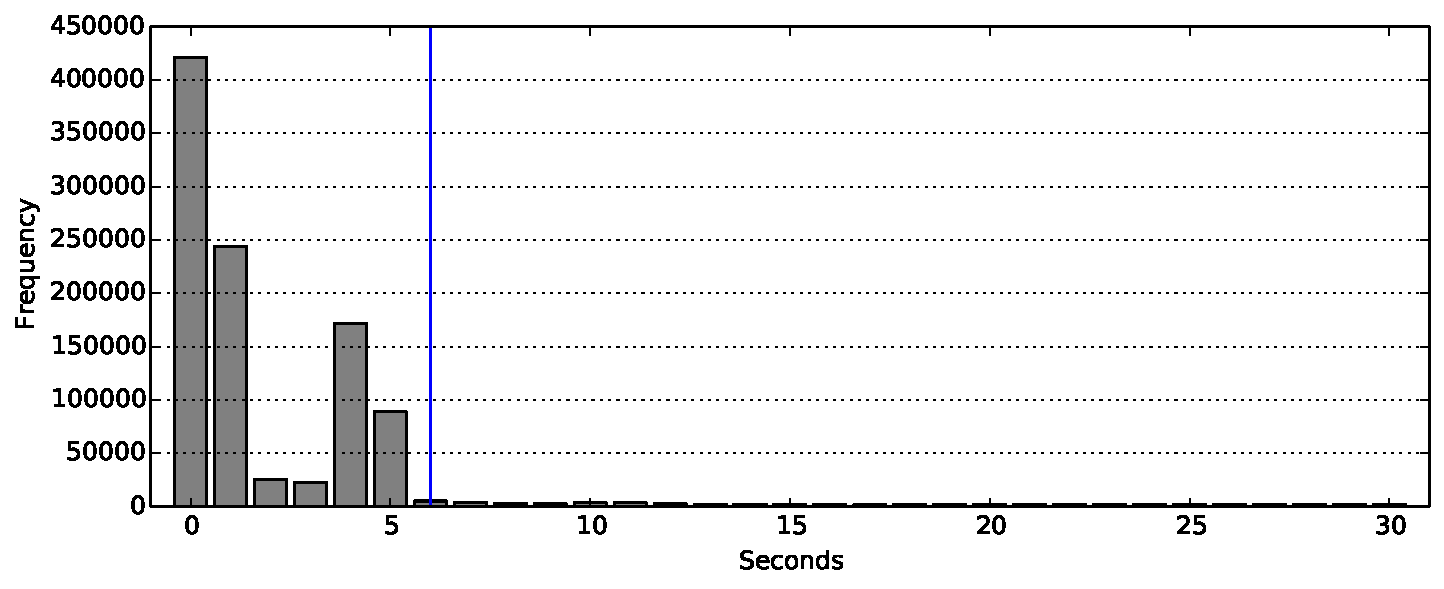
\includegraphics[width=\textwidth]{../result/2015-08-14_17-46-44_faui1-246_timeout}
\caption[Duration of receiving one peer message]{Duration of receiving one peer message. Data is taken from files \texttt{2015-08-14\_17-46-44\_faui1-246.sqlite} and \texttt{2015-08-14\_17-46-44\_faui1-246\_timeout.txt}.}
\label{timeout-calibration}
\end{figure}

To assess a minimum timeout, an analysis with special configuration parameters was performed. Here, the maximum time used for receiving one message was recorded for every peer contact. These durations were rounded and the number of occurrences plotted in figure \ref{timeout-calibration}. For this task \config{network\_timeout} was set to 30 seconds to achieve most unbiased results. During this test at \numprint{977301} out of \numprint{1040817} peer contacts the maximum duration for receiving one message was below six seconds, which equals \numprint[\%]{93.9}. The recording of this value can be enabled with \config{rec\_dur\_analysis}.

\paragraph{receive\_message\_max}
When collecting all messages from a peer, a maximum of \numprint{256} messages are considered. This limit is in place, to prohibit infinite peer sessions. Only *\numprint[\%]{0} of evaluations reached this maximum on the main analysis pass, others stopped because of the timeout or another error.

\paragraph{peer\_revisit\_delay}
Peers were contacted for their download progress every five minutes. This delay should be as small as possible, to also consider peers who stop seeding a torrent immediately after they finished downloading it. Five minutes caused no problem with system resources.

\paragraph{tracker\_request\_interval and dht\_request\_interval}
Both request intervals were set to five minutes. As discussed later in section \ref{addr}, the rates of doubly received peers are very high. This shows five minutes is enough to cover the majority of peers.

\paragraph{torrent\_complete\_threshold}
This is actually just the threshold, where the analysis module stops to keep track of a peer and will no longer contact him. The threshold used for confirmed download calculation can be chosen separately when compiling download numbers from the database. However, the threshold for download counting must be equal or lower than this threshold, because peers above were not tracked in the first place. The value of \numprint[\%]{98} was chosen, because peer's progress appeared often to stop between \numprint[\%]{98} and \numprint[\%]{100}. So \numprint[\%]{+-2} seems to be the precision of the measured download progress. This suggests, that a threshold above \numprint[\%]{98} causes traffic without further benefits.

\paragraph{peer\_evaluation\_threads}
This is the number of threads who are contacting peers from the \emph{peer queue}, which contains addresses from tracker servers and the DHT network. In this analysis \numprint{1024} threads were used. Every peer evaluation needs at least six seconds, because the message receiving has to time out. In order to process peers quickly, many threads are needed. Since threads are mostly idle waiting for a timeout, this number of threads is not a problem for system load.

\section{Restrictions}
\label{rest}
To get most complete results, the BitTorrent Download Analyzer aims to collect data from as many peers as possible. Unfortunately, there are still a few restrictions regarding peer sources in comparison to real BitTorrent clients. This is due to the high implementation and development effort which would be necessary to integrate each of those. For each restriction it will be discussed shortly, why it does not harm this work at large.
\begin{itemize}
\item No support for IPv6 addresses from HTTP announce requests \cite{bep7} or the separate IPv6 DHT network \cite{bep32}. A measurement study \cite[sec.~4.2.]{vyncke2012measuring} from 2011 for IPv6 traffic in BitTorrent networks found between \numprint[\%]{1} and \numprint[\%]{4} of peers using IPv6.
\item No support for the Micro Transport Protocol ($\mu$TP or uTP) \cite{bep29}, which enables UDP communication between peers. Peers can support this in addition to the Peer Wire Protocol for better bandwidth management. Users can configure clients to only use uTP, but this may harm their download speeds.
\item No support for peer exchange (PeX). This enables peers to exchange peer lists among each other with simple messages. Currently there are different implementations in use, an official BEP does not exist, yet.
\item No support for the Tracker exchange extension \cite{bep28}, which enables peers to exchange announce URLs of tracker servers. This is useful for magnet links without any trackers or torrent files with missing trackers. All torrents investigated in this work have at least *\numprint{0} trackers, see section \ref{addr}.
\item No support for the Azureus DHT network, which is a separate DHT network from \emph{Mainline DHT} described in \cite{bep5}. Peer numbers in the Azureus DHT network are significantly lower \cite[table~5]{drachen2011distribution}.
\end{itemize}
%%%%%%%%%%%%%%%%%%%%%%%%%%%%%%%%%%%%%%%%%%%%%%%%%%%%%%%%%%%%%%%%%%%%%%%%%%%%%%%%%

\chapter{Evaluation}
\label{eval}
Data collection with the BitTorrent Download Analyzer tool was performed simultaneously on two identical virtual machines running Ubuntu 14.04 LTS with 2.0\,GB of RAM, 3.4\,GHz dual-core processors and own IPv4 addresses without NAT. The analysis was performed for \numprint{34} hours \range. Each machine was running an own \emph{pymdht} DHT node, which did not crash before or during the analysis. The BitTorrent Download Analyzer gave no problematic error messages in the logfile. The used BitTorrent port was changed right before the evaluation started, in order to decrease system load from peers with an unrelated info hash from earlier evaluations.

\begin{figure}
\centering
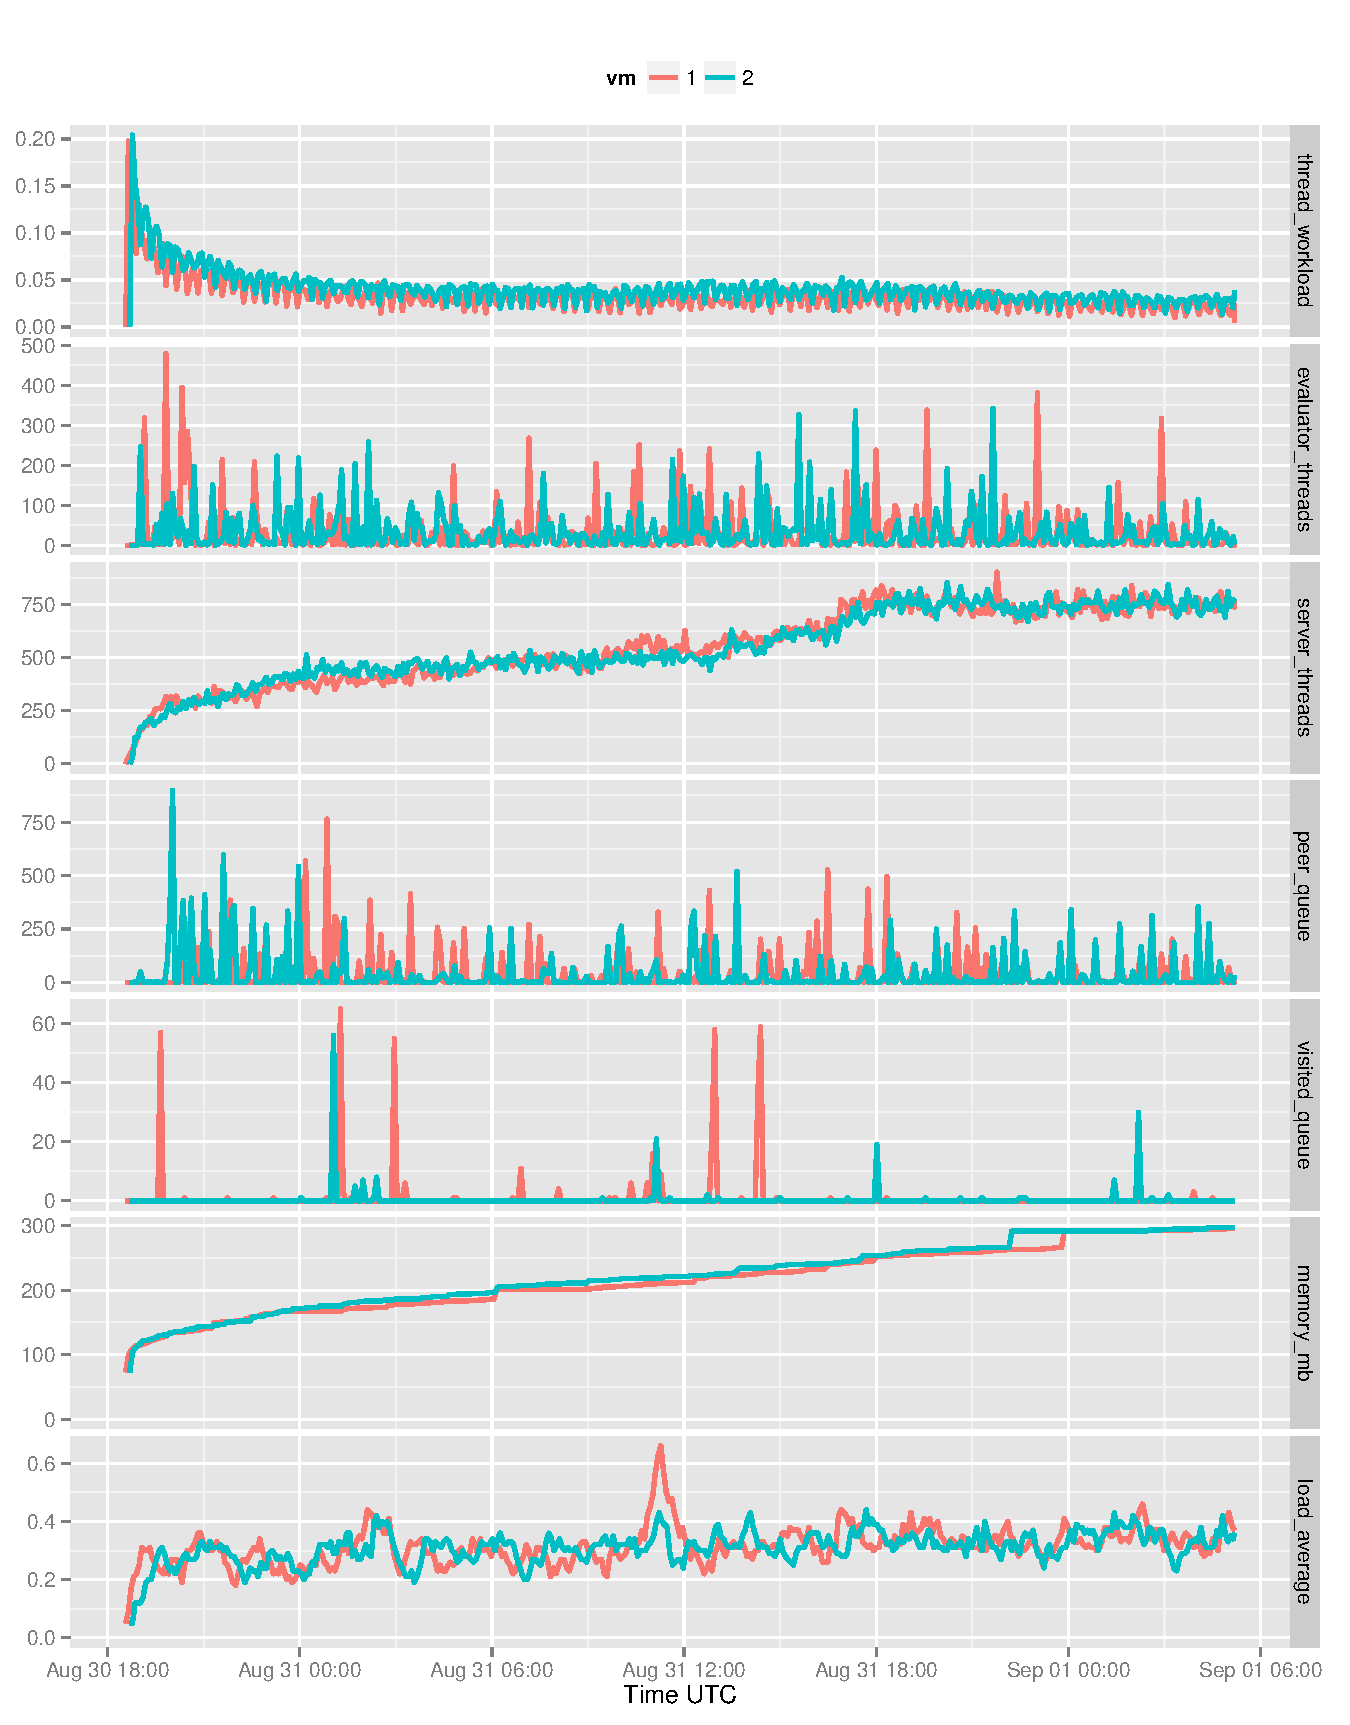
\includegraphics[width=\textwidth]{../result/2015-08-30_20-combined_workload}
\caption[Monitoring parameters during the analysis]{System parameters and queue lengths for monitoring. The \emph{thread workload} is a time based value between \numprint{0} and {1}, stating the average uptime of the peer contact threads, not the server threads. A thread is only considered as inactive when waiting on an empty \emph{peer queue} or waiting for the revisiting timestamp of a peer, see section \ref{cont}. The \emph{evaluator threads} graph gives the same value as an absolute number while using the same constraints. \emph{Server threads} is the number of active server threads, which is not limited. \emph{Peer queue} and \emph{visited queue} are the lengths of these queues. \emph{Memory MB} specifies RAM usage, \emph{load average} is the standard Unix processor load parameter.}
\label{workload}
\end{figure}

In order to support the validity of the test results, some statistics were logged to the database with a sample rate of five minutes. These are shown in figure \ref{workload}. Graphs of a low thread workload and the short length of the peer queue make clear, that the number of \numprint{1024} worker threads was enough. The number of used evaluator threads did actually not surpass \numprint{500}. The length of the visited queue is almost always zero, which proves that the database was not a bottleneck. A maximum of \numprint[MB]{300} RAM is used, which is way below the available \numprint[GB]{2}. The Unix load-average is below the \numprint{2} mark for two processor cores.

After the development phase of the BitTorrent Download Analyzer was finished, the \emph{SQLAlchemy} database toolkit started to report errors about a locked database. This occurred despite using the multi-threading mechanisms provided by SQLAlchemy. The problem surfaced very late and could not be resolved because of this. The errors were only reported for the request table and the statistic table for monitoring values and were few in comparison to the number of successfully stored database rows. The used workaround for this problem was to apply failed SQL statements, which were all recorded in the logfile, to the database afterwards. Finally, the databases of the two virtual machines were combined. The commands used for creating the final database are given in listing \ref{magic}.
\begin{lstlisting}[language=bash, otherkeywords={scp, sqlite3}, float, caption={[Creating the final database]Steps to create the final database. The \texttt{combine.sql} scripts produces \texttt{INSERT} statments for all table rows of both databases and handles torrent IDs appropriately. Filename timestamps are in CEST, which is UTC+02:00. \texttt{2015-08-30\_20-combined.sqlite} holds the data used for the evaluation.}, captionpos=b, label=magic]
scp torrent-vm1:bittorrent-analyzer/btda/output/2015-08-30_20-34-06_faui1-246* .
scp torrent-vm2:bittorrent-analyzer/btda/output/2015-08-30_20-41-36_faui1-246* .
./sql_from_log.py 2015-08-30_20-34-06_faui1-246.log
./sql_from_log.py 2015-08-30_20-41-36_faui1-246.log
cat 2015-08-30_20-34-06_faui1-246.log.sql | sqlite3 2015-08-30_20-34-06_faui1-246.sqlite
cat 2015-08-30_20-41-36_faui1-246.log.sql | sqlite3 2015-08-30_20-41-36_faui1-246.sqlite
cat combine.sql | sqlite3 | sqlite3 2015-08-30_20-combined.sqlite
\end{lstlisting}

\section{Choosing Torrents}
\label{cho}
\begin{table}
\centering
\begin{tabular}{rllr}
\toprule
Rank & Site name & Domain name & Alexa Rank \\
\midrule
1 & Kickass Torrents & \texttt{kat.cr} & 116 \\
2 & ExtraTorrent.cc & \texttt{extratorrent.cc} & 335 \\
3 & Nyaa Torrents & \texttt{www.nyaa.se} & 399 \\
4 & Torrentz Search Engine & \texttt{torrentz.eu} & 464 \\
5 & The Pirate Bay & \texttt{thepiratebay.se} & 507 \\
6 & YTS & \texttt{yts.to} & 669 \\
7 & Rarbg & \texttt{rarbg.to} & 1,150 \\
8 & 1337x & \texttt{1337x.to} & 1,661 \\
9 & EZTV & \texttt{eztv.ch} & 1,831 \\
10 & torrentHound.com & \texttt{www.torrenthound.com} & 2,188 \\
11 & IPTorrents & \texttt{iptorrents.com} & 3,256 \\
12 & isoHunt & \texttt{isohunt.to} & 3,816 \\
13 & Bitsnoop P2P Search & \texttt{bitsnoop.com} & 4,293 \\
14 & Torrent Downloads & \texttt{www.torrentdownloads.me} & 4,315 \\
15 & LimeTorrents.cc & \texttt{www.limetorrents.cc} & 4,552 \\
16 & TamilRockers.net & \texttt{tamilrockers.com} & 4,586 \\
17 & Monova Torrent Search & \texttt{www.monova.org} & 4,843 \\
\bottomrule
\end{tabular}
\caption[Popular torrent directory sites according to \textsc{Alexa}]{Popularity of torrent directory sites according to \textsc{Alexa}'s \cite{alexa} global traffic ranking. Only sites with a rank below \numprint{5000} are listed. Data is accurate as of July 16, 2015.}
\label{torrentsites}
\end{table}

Due to the distributed nature of BitTorrent, there is no complete list of all active torrents. External data about popularity of torrents is needed, even if there is no guarantee of completeness. To get an overview about torrent directory sites and determine the most popular ones, the global traffic rankings by \textsc{Alexa Internet, Inc.} \cite{alexa} were consulted. The websites where \textsc{Alexa}'s ranking was looked up were collected through manual investigation using web search engines, relevant news sites and cross references between torrent sites. Table~\ref{torrentsites} shows the \numprint{17} sites found having an rank below \numprint{5000}.

\begin{table}
\centering
\begin{tabular}{lrlrrr}
\toprule
Set & ID & Name & Pieces & Size & Trackers \\
\midrule
Set A & 17 & [ www.CpasBien.pw ] Avengers.Age... & \numprint{5619} & \numprint[GB]{1.47} & 10 \\
& 8 & Magic.Mike.XXL.2015.HDRip.XViD.A... & \numprint{1426} & \numprint[GB]{1.50} & 10 \\
& 12 & San.Andreas.2015.HDRip.XviD.AC3-... & \numprint{5880} & \numprint[GB]{1.54} & 10 \\
& 4 & Minions.2015.720p.HDRip.X264.AAC... & \numprint{3980} & \numprint[GB]{2.09} & 10 \\
& 13 & San Andreas 2015 720p WEB-DL x26... & \numprint{610} & \numprint[GB]{2.56} & 10 \\
& 15 & Mission.Impossible.5-Rogue.Natio... & \numprint{11798} & \numprint[GB]{3.09} & 10 \\
& 3 & Straight.Outta.Compton.2015.1080... & \numprint{4108} & \numprint[GB]{4.31} & 7 \\
& 5 & Avengers.Age.of.Ultron.2015.720p... & \numprint{4369} & \numprint[GB]{4.58} & 7 \\
Set B & 11 & Avengers Age of Ultron 2015 1080... & \numprint{1327} & \numprint[GB]{5.57} & 10 \\
& 9 & F3\_GOTY.iso & \numprint{1848} & \numprint[GB]{7.75} & 5 \\
& 19 & Game.Of.Thrones.S05.Season.5.COM... & \numprint{2270} & \numprint[GB]{9.52} & 5 \\
& 18 & 3DMGAME-One.Piece.Pirate.Warrior... & \numprint{2657} & \numprint[GB]{11.14} & 5 \\
& 16 & DRP\_15.8\_Full.iso & \numprint{10711} & \numprint[GB]{11.23} & 5 \\
& 2 & Narcos S01 720p WEBRip x264-TAST... & \numprint{1826} & \numprint[GB]{15.32} & 10 \\
Set C & 1 & Battlefield Hardline by xatab & \numprint{3599} & \numprint[GB]{30.19} & 7 \\
& 20 & Mortal.Kombat.X.Proper-RELOADED & \numprint{3998} & \numprint[GB]{33.54} & 5 \\
& 10 & The X-Files S01-S09 WEBRip x264-... & \numprint{12502} & \numprint[GB]{52.44} & 10 \\
& 14 & Batman.Arkham.Knight-CPY & \numprint{6430} & \numprint[GB]{53.94} & 10 \\
& 7 & Dexter Season 1, 2, 3, 4, 5, 6, ... & \numprint{7774} & \numprint[GB]{65.21} & 10 \\
\bottomrule
\end{tabular}
\caption[List of torrent chosen for evaluation]{List of 19 popular torrents according to meta-search engine \textsc{Torrentz} \cite{torrentz}. The selection was made \numprint{30} minutes before the analysis started. The \emph{ID} was chosen by the SQLite database. Some movies are shared in multiple active torrents, but have different sizes or were uploaded by different users.}
\label{torrents}
\end{table}

Popular torrents were often found to be registered on multiple tracker sites, which leads to mostly identical top torrents across these torrent sites. For the definite selection of torrents, the meta-search engine \textsc{Torrentz} \cite{torrentz} was used: It monitors torrents from all other major torrent sites and provides sorting and filter options by peer count, torrent age and size.
Torrents of various sizes between \numprint[GB]{1.5} and \numprint[GB]{65} were chosen, because the torrent size has high influence on further results. For further reference, three size groups are defined. These three sets will be evaluated separately where appropriate.
\begin{itemize}
\item Set A: Between \numprint[GB]{1} and \numprint[GB]{5}
\item Set B: Between \numprint[GB]{5} and \numprint[GB]{20}
\item Set C: Between \numprint[GB]{30} and \numprint[GB]{70}
\end{itemize}

In order to observe many downloads, torrents with high amount of leechers were selected. Initially \numprint{20} torrents were chosen, but one tracker the torrent with ID 6 sent a bencoded value, which was not standard conform as described in section \ref{bittorrent}. This crashed the tracker request thread for this torrent, which is why this torrent is excluded from the evaluation. The 19 remaining torrents are listed in table \ref{torrents}. A metainfo file was available for all torrents.

\section{Getting Addresses of Peers}
\label{addr}
\begin{table}
\centering
\begin{tabular}{lrrr}
\toprule
Source & Total & Unique & New \\
\midrule
Tracker server & \numprint{5614412} & \numprint{691248} & \numprint[\%]{12.31} \\
DHT network & \numprint{3546070} & \numprint{856367} & \numprint[\%]{24.15} \\
Incoming peers & \numprint{6538653} & \numprint{258939} & \numprint[\%]{3.96} \\
\emph{Total} & \numprint{15699135} & \numprint{1806554} & \numprint[\%]{11.51} \\
\bottomrule
\end{tabular}
\caption[Received peer addresses per source]{Total and unique received peer addresses per source for all torrents. The ratio of new \emph{tracker} and \emph{DHT} peers depends mainly on the request interval for new peers. Numbers of \emph{incoming peers} only include those where the download progress was evaluated successfully. Numbers of \emph{total} received peers may overlap between sources in this table. Numbers of \emph{unique} peers do not overlap between sources, each peer is only counted as unique one time. This is why the distribution between sources may not represent uniqueness per source in general, but only in this data set. Numbers were acquired from the \emph{request} database table.}
\label{unique-peers}
\end{table}
% SQL Total: select sum(received_peers) from request where source='<source>';
% SQL Unique: select sum(received_peers) - sum(duplicate_peers) from request where source='<source>';

Peers from all supported sources were considered, namely from the tracker server, the DHT network and incoming connections. The total number collected addresses across all torrents during this analysis in regards to their source is shown in table \ref{unique-peers}. The overall high rates of duplicate peers reveal, that the majority of peers collectable through these sources was received. The \emph{incoming peers} data point in this table only includes peers, when their download progress was successfully evaluated. Hence, the ratio of \numprint[\%]{3.96} new incoming peers implies that \numprint[\%]{96.04} of all incoming contacts are second or later visits, although peers did not receive any torrent data. Only these later visits allow to determine the crossing of a threshold.

\begin{figure}
\centering
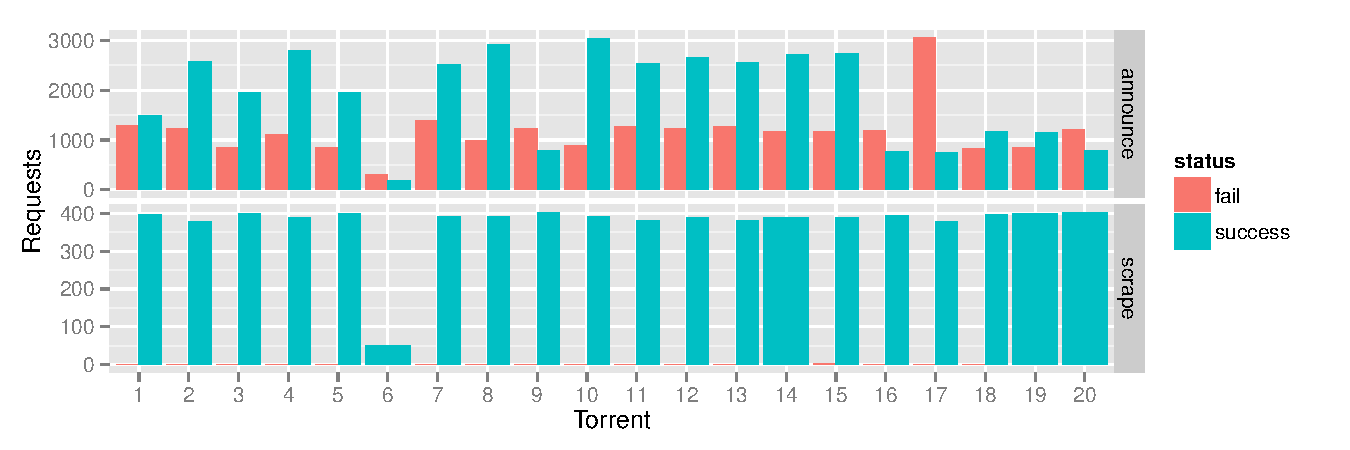
\includegraphics[width=\textwidth]{../result/2015-08-30_20-combined_tracker-error}
\caption[Responsiveness of tracker servers per torrent]{Responsiveness of tracker servers per torrent. The thread to perform announce requests for torrent 6 crashed after four hours, which is why this torrent is excluded from the analysis. As apparent from table \ref{torrents}, metainfo files for torrents 9, 16 and 18 to 20 had only five announce URLs embedded, explaining the reduced request numbers. Also torrents 1, 3 and 5 only had seven trackers. Data is taken from the file \texttt{2015-08-30\_20-combined\_tracker-error.txt}, which is written by the analyzer tool.}
\label{tracker-resp}
\end{figure}

The responsiveness of the trackers per torrent is examined in figure \ref{tracker-resp}. As expected, torrents with less tracker announce URLs embedded in the torrent file show less attempted announce requests. From torrents with ten trackers usually about two third of them respond. On torrents with only five announce URLs about half of them responded. Torrent 17 stands out with a high number of failed requests. Reviewing the logfile reveals, that only two out of ten trackers responded. Other trackers may have been unreliable or actually removed the torrent due to a DMCA takedown notice by the copyright owner.

\begin{figure}
\centering
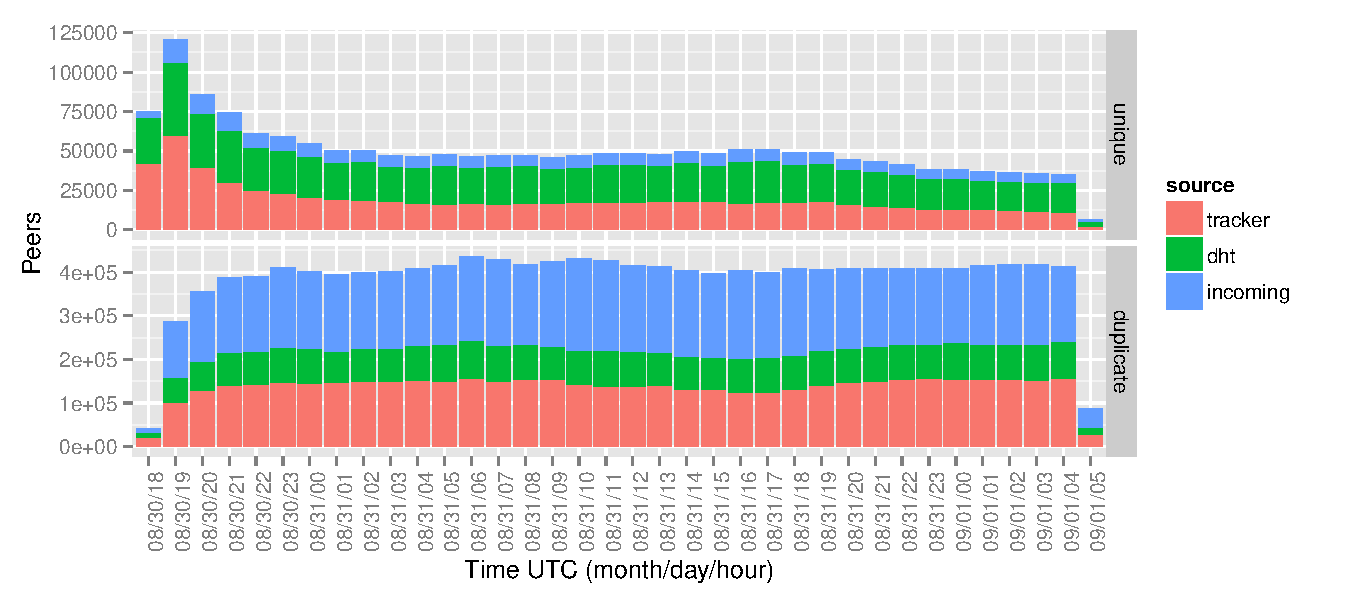
\includegraphics[width=\textwidth]{../result/2015-08-30_20-combined_source_all_torrents}
\caption[Development of received peer addresses per source]{Development of received peer addresses per source for all torrents. UDP trackers returned always \numprint{200} addresses per request, trackers with HTTP access \numprint{50}. Torrents are usually registered with a few trackers. DHT request were observed to return between \numprint{100} and \numprint{1300} peers each. Values have the same characteristics as described in table \ref{unique-peers}: \emph{Incoming} peers only include successfully evaluated ones, \emph{unique} peers do not overlap between sources, \emph{duplicate} peers may overlap between sources. The unique peers diagram uses a smaller scale for peers than the duplicate ones to increase its readability.}
\label{request-history}
\end{figure}

The number of new collected unique peer addresses is highest in the first few hours, as shown in the the summary for all torrents  in figure \ref{request-history}. Nearly all peers in the first \numprint{30} minutes are new. The value declines and stays steady at \numprint{50000} unique peers per hour for about \numprint{18} hours. In the last \numprint{15} hours of the analysis, this value declines slowly. The spike at the beginning consists of all peers in the torrent swarm at this point in time. The constant part are new peers who enter the torrent during the analysis period. The decline at the end may be users loosing interest of the torrent's contents, because other torrents raise in popularity. Another valid explanation is a 24-hour cycle, which implies that unique peer numbers would raise again later. The duration of \numprint{34} hours is too short to tell the difference.

\section{Counting Confirmed Downloads}
\subsection{Trying Different Thresholds}
\begin{figure}
\centering
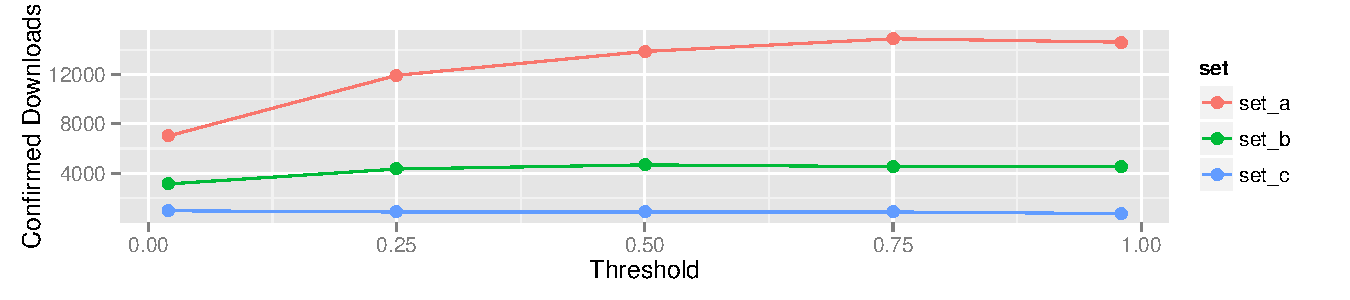
\includegraphics[width=\textwidth]{../result/2015-08-30_20-combined_threshold}
\caption[Confirmed downloads using different thresholds]{Confirmed downloads using different thresholds per torrent set. Peers with pieces on the first visit below and on the last visit above the threshold are counted as confirmed.}
\label{thresh-chg}
\end{figure}

Peers were tracked up to a download progress of \numprint[\%]{98}. Since the number of pieces on the first and last contact for each peer was recorded, the number of confirmed downloads can be extracted by filtering for peers with a progress on the first visit below and on the last visit above the threshold. Different threshold values were tested in figure \ref{thresh-chg}. The maximum value of calculated downloads is nearly identical between \numprint[\%]{75} and  \numprint[\%]{98}, with declining numbers for lower thresholds. The value of \numprint[\%]{98} will be used for the further evaluation, in order to only register complete downloads.

\subsection{Summary}
\begin{table}
\centering
\begin{tabular}{lrrrrrr}
\toprule
Set & Confirmed & Reported & Unique Peers & C./R. & C./U. & R./U. \\
\midrule
Set A & \numprint{14632} & \numprint{150629} & \numprint{1264472} & \numprint[\%]{9.71} & \numprint[\%]{1.16} & \numprint[\%]{11.91} \\
Set B & \numprint{4505} & \numprint{17872} & \numprint{383420} & \numprint[\%]{25.21} & \numprint[\%]{1.17} & \numprint[\%]{4.66} \\
Set C & \numprint{713} & \numprint{1299} & \numprint{158662} & \numprint[\%]{54.89} & \numprint[\%]{0.45} & \numprint[\%]{0.82} \\
\emph{Total} & \numprint{19850} & \numprint{169800} & \numprint{1806554} &\numprint[\%]{11.69} & \numprint[\%]{1.10} & \numprint[\%]{9.40} \\
\bottomrule
\end{tabular}
\caption[Confirmed downloads per torrent set]{Confirmed downloads per torrent set. Two comparison values are given: \emph{Reported} downloads are the differences from the number of completed downloads in a tracker's scrape response. \emph{Unique peers} is the number of unique peer addresses collected in the process.}
\label{confirmed-downloads}
\end{table}

To judge the success of counting confirmed downloads with the planned method, two comparison values will be considered. First, the number of completed downloads as reported by the tracker server. This is a value available form the tracker through scrape requests, which were issued regularly together with announce requests. For each hour, the difference of this value was calculated. As stated in section \ref{req}, scrape requests were only issued to the main tracker embedded in the torrent file, since the numbers may overlap between trackers otherwise. The second comparison value is the number of collected unique peer addresses as introduced in table \ref{unique-peers}. This may include outdated information of peers who have disconnected meanwhile or never finished the download. Both values can not provide the true number of happened downloads, but allow to assess the performance of the tool. Table \ref{confirmed-downloads} shows the comparison values per torrent set. Following conclusions are possible:
\begin{enumerate}
\item The number of total unique peers is way above confirmed and reported downloads, roughly by factor 100 and 10 respectively.
\item Judging by tracker reported numbers, confirmed downloads are more accurate with larger torrents.
\item For large torrents, there are less reported downloads per unique peer than for small ones.
\end{enumerate}

\begin{figure}
\centering
{\small (a) Confirmed downloads by reported downloads.}
\includegraphics[width=\textwidth, page=2]{../result/2015-08-30_20-combined_download_confirmed_scrape}
{\small (b) Confirmed ratio regarding reported downloads by torrent size.}
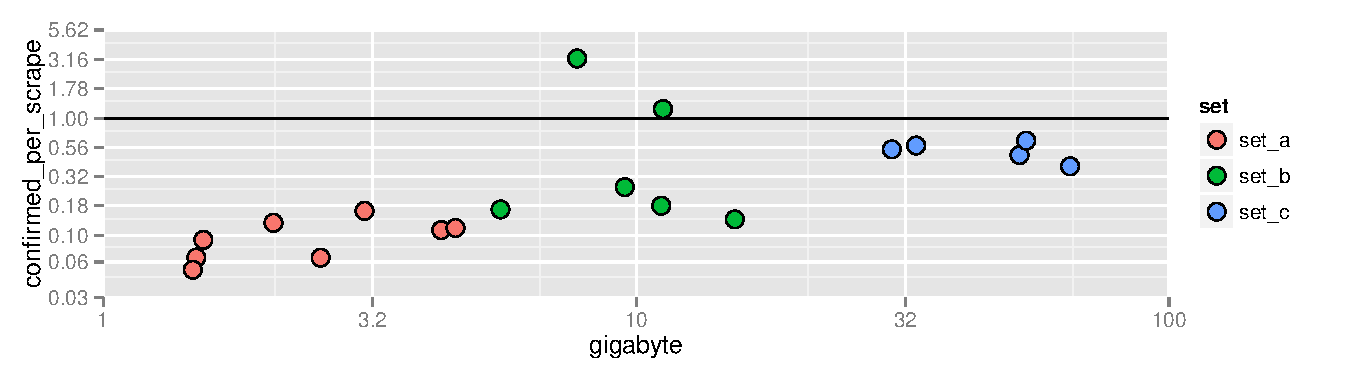
\includegraphics[width=\textwidth, page=1]{../result/2015-08-30_20-combined_download_confirmed_scrape}
\caption[Download numbers: Confirmed vs. scrape request]{Relation between confirmed downloads and tracker reported download numbers from scrape requests per torrent, using a double logarithmic scale. Each point represents a torrent. The black lines mark the identity between confirmed and reported downloads.}
\label{confirmed-scrape}
\vspace{1cm}
{\small (a) Confirmed downloads by unique peers.}
\includegraphics[width=\textwidth, page=2]{../result/2015-08-30_20-combined_download_confirmed_unique}
{\small (b) Confirmed ratio regarding unique peers by torrent size.}
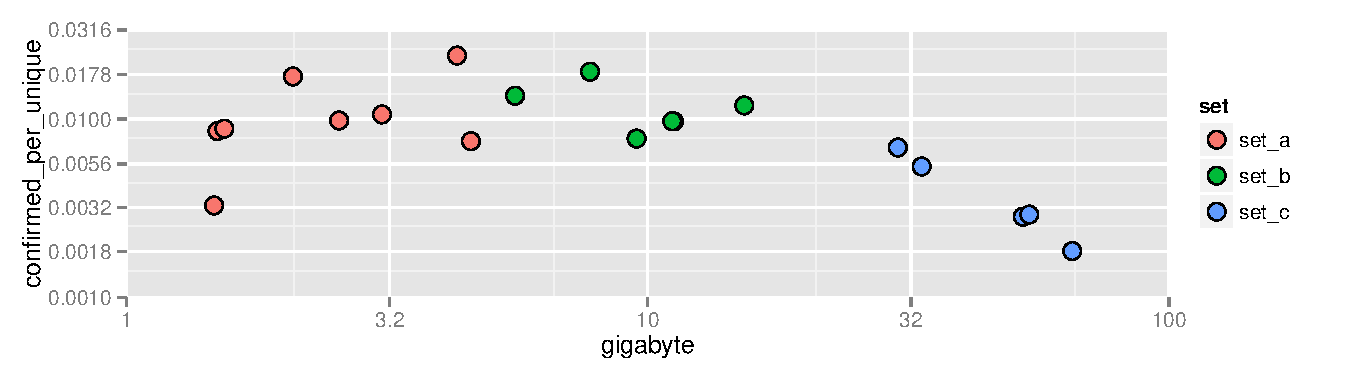
\includegraphics[width=\textwidth, page=1]{../result/2015-08-30_20-combined_download_confirmed_unique}
\caption[Download numbers: Confirmed vs. unique peers]{Relation between confirmed downloads and unique collected peer addresses per torrent, using a double logarithmic scale. Each point represents a torrent. The identity between confirmed downloads and unique peers is outside of the plot area.}
\label{confirmed-unique}
\end{figure}

\subsection{Comparison with Scrape Requests}
When viewing data for each torrent in figure \ref{confirmed-scrape} (a), a clear positive relation between confirmed downloads and tracker reported numbers is visible, although confirmed numbers are mostly lower. It is also obvious, that large torrents are less downloaded than smaller ones in general. Part (b) plots the success rates of measuring confirmed downloads, using the tracker's scrape numbers as a reference. The chart shows, that for torrents in set A with less than \numprint[GB]{5}, the numbers of confirmed downloads are only between \numprint[\%]{4} and \numprint[\%]{17}. Results between \numprint[GB]{5} and \numprint[GB]{20} in set B are all above \numprint[\%]{13}. On two torrents, the measured numbers exceed the tracker reported ones by factor \numprint{1.2} and {3.2}. All five large torrents of set C are between \numprint[\%]{39} and \numprint[\%]{64} percent. These graphs shows three things:
\begin{enumerate}
\item Confirmed download numbers produced by the BitTorrent Download Analyzer are heavily correlated with tracker reported complete downloads.
\item The method of counting confirmed downloads is heavily dependent on the torrent size. Best results above \numprint[\%]{40} are achieved with torrents above \numprint[GB]{30}. Presumably, the reason for this is the increased likelihood of recording a peer's download progress, when the downloads takes more time. This is given with large torrents.
\item Scrape requests are not always accurate and can indicate too small download numbers. This is understandable, since the tracker relies on every peer to report a finished download. A BitTorrent client may disconnect without sending an \emph{completed} event to the server. A client may not have used the main tracker of the torrent in the first place, but another one or none at all.
\end{enumerate}

\subsection{Comparison with Unique Peers}
In figure \ref{confirmed-unique} similar data is shown, but using the number of collected unique peer addresses as a reference. When considering part (a), a correlation between the number of unique peers and the number of confirmed downloads is still recognizable, although unique peer numbers are way higher than confirmed downloads. This was already apparent from table \ref{confirmed-downloads}. Again, success rates of counting confirmed downloads are given by torrent size in part (b). In this graph, the success rate of set C is noticeable low, which contradicts with the scrape-based success rate discussed above. However, the success rate based on unique peers is tiny for all torrents and varies between \numprint[\%]{0.1} and \numprint[\%]{2.3}. This is too small to draw conclusions. We can learn from this data:
\begin{enumerate}
\item Confirmed download numbers are also heavily correlated with the number of unique peers collected by the BitTorrent Download Analyzer.
\item The success rate of confirming downloads for unique peers is below \numprint[\%]{3}. An important reason for this are seeding peers, which are part of the torrent swarm, but do not download any more. Besides this, outdated peer data reduces this value.
\item The smallest number of confirmed downloads per unique peer was determined for torrents above \numprint[GB]{30}. This matches with the comparison between tracker reported downloads and observed peer addresses in table \ref{confirmed-downloads}.
\end{enumerate}

\subsection{Downloads per Hour}
\begin{figure}
\centering
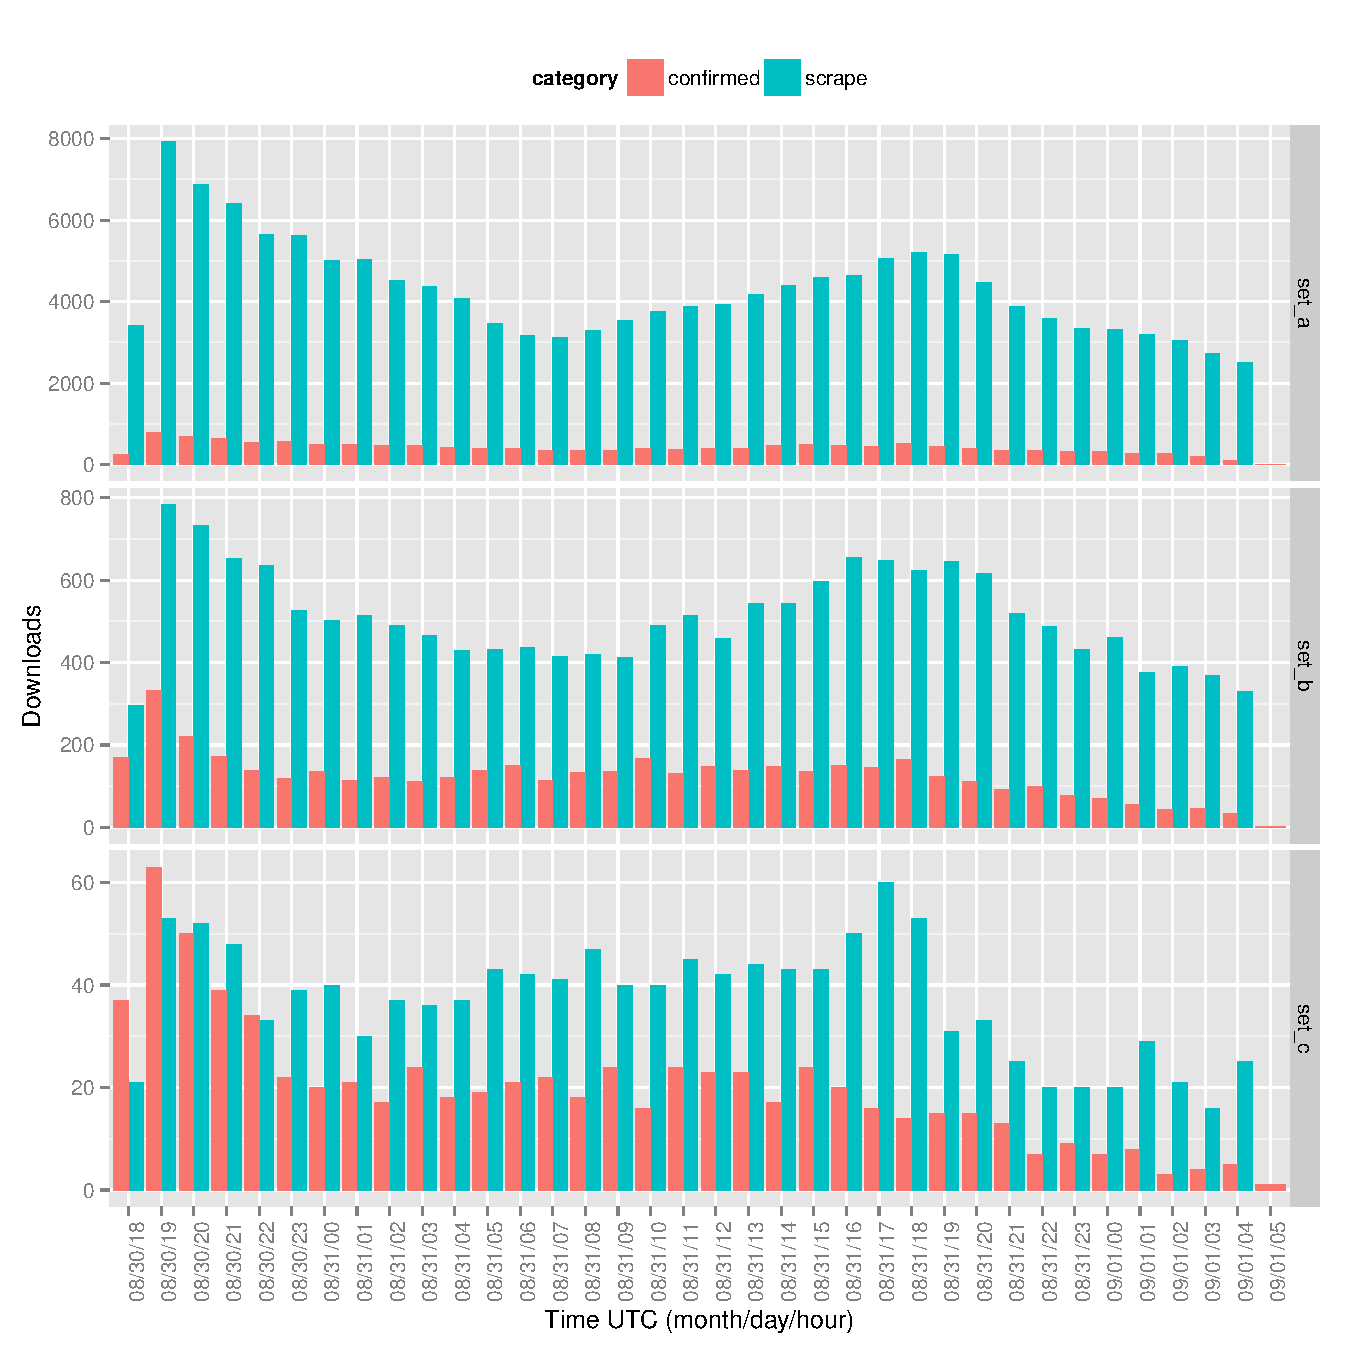
\includegraphics[width=\textwidth]{../result/2015-08-30_20-combined_download_set}
\caption[Development of confirmed and reported downloads]{Development of confirmed and server reported downloads per hour and torrent set. The timestamp for a confirmed download is the time of first contact with the peer. Analysis duration was \range.}
\label{download-history}
\end{figure}

The history of download numbers over time in figure \ref{download-history} once more illustrates the relation between measured download numbers and torrent size. Unfortunately in retrospect, the timestamp when a peer crossed the download threshold was not recorded, but only one from the first and the last contact. In this plot, the time of first contact is used, which explains the high numbers in the beginning and low values at the end. Likewise to the received peer addresses in figure \ref{request-history}, download numbers settle after a few hours.

\section{Problems}
\label{problems}
\begin{table}
\centering
\begin{tabular}{llrr}
\toprule
Event & Result & Frequency & Share per Event \\
\midrule
First contact & Timed out & \numprint{978505} & \numprint[\%]{61.40} \\
 & Connection refused & \numprint{242616} & \numprint[\%]{15.22} \\
 & Socket connection broken & \numprint{177833} & \numprint[\%]{11.16} \\
 & Success & \numprint{149608} & \numprint[\%]{9.39} \\
 & No route to host & \numprint{22042} & \numprint[\%]{1.38} \\
 & Connection reset by peer & \numprint{21512} & \numprint[\%]{1.35} \\
 & Network is unreachable & \numprint{1446} & \numprint[\%]{0.09} \\
 & Peer speaks unknown protocol & \numprint{24} & \numprint[\%]{0.00} \\
 & \emph{Total} & \numprint{1593586} & \\
\midrule
Later contact & Success & \numprint{166174} & \numprint[\%]{81.74} \\
 & Socket connection broken & \numprint{26559} & \numprint[\%]{13.06} \\
 & Timed out & \numprint{7203} & \numprint[\%]{3.54} \\
 & Connection reset by peer & \numprint{1725} & \numprint[\%]{0.85} \\
 & Connection refused & \numprint{1252} & \numprint[\%]{0.62} \\
 & No route to host & \numprint{390} & \numprint[\%]{0.19} \\
 & Network is unreachable & \numprint{5} & \numprint[\%]{0.00} \\
 & \emph{Total} & \numprint{203308} & \\
\midrule
Incoming peer & Unknown info hash & \numprint{7187788} & \numprint[\%]{37.26} \\
 & Already in outgoing & \numprint{6572026} & \numprint[\%]{34.07} \\
 & Peer speaks unknown protocol & \numprint{2283818} & \numprint[\%]{11.84} \\
 & Timed out & \numprint{2144463} & \numprint[\%]{11.12} \\
 & Success & \numprint{1059055} & \numprint[\%]{5.49} \\
 & Connection reset by peer & \numprint{26330} & \numprint[\%]{0.14} \\
 & Socket connection broken & \numprint{16266} & \numprint[\%]{0.08} \\
 & Broken pipe & \numprint{2} & \numprint[\%]{0.00} \\
 & \emph{Total} & \numprint{19289748} & \\
\bottomrule
\end{tabular}
\caption[Reasons for failure of peer evaluation]{Outcome of peer evaluations for different events. An \emph{event} describes the point in the evaluation process. \emph{First} and \emph{later contact} are performed when actively contacting collected peer addresses. After an evaluation of a peer fails, the peer is not contacted another time. An \emph{incoming peer} represents an incoming connection on the BitTorrent listening port. Error data is from the \texttt{2015-08-30\_20-combined\_peer-error.txt} file as written by the analyzer tool, success counts are from the \emph{visits} column of the \emph{peer} table.}
\label{connection-failure}
\end{table}
% SQL success first: select count(visits) from peer where source='tracker' or source='dht';
% SQL success later: select sum(visits-1) from peer where source='tracker' or source='dht';
% SQL success incoming: select count(visits) from peer where source='incoming';

\begin{figure}
\centering
\includegraphics[width=\textwidth, page=2]{../result/2015-08-30_20-combined_visits}
\caption[CDF of successful peer visits per source]{CDF of successful peer visits per source. Only peers of which the download progress was evaluated successfully at least once are included in this figure. A lower graph is better as it indicates more visits per peer. Most of the peers who were contacted actively could only be visited once. Incoming peers try to get pieces usually a few times, while many of them stop trying after the first or the eighth attempt. Some even never stop trying.}
\label{visits}
\end{figure}

The Evaluation of a peer's download progress was described in section \ref{peer-evaluation}. This process can fail for various reasons. The superficial problems which occurred in this analysis are listed in table \ref{connection-failure}. The table shows every attempt of connecting to a peer and performing the evaluation procedure. It shows, that the chance of successfully evaluating a peer's download progress on first contact is \numprint[\%]{9.4}. The majority of connection attempts timed out. The number of \numprint[\%]{82} succeeded later evaluation attempts seems to indicate a high success rate when contacting a peer a second time. However, one has to consider, that a peer is not contacted ever again after a failed attempt. This means every error on a later contact is a lost peer, successful evaluations were performed multiple times per peer. The effect is obvious when viewing figure \ref{visits}: After one successful visit, the chance of a second successful visit is only about \numprint[\%]{15}.

Regarding incoming connections, most evaluations failed due to an unknown info hash. Before the data of this evaluation was collected, the analysis tool was tested with different torrents on BitTorrent port \numprint{6883}. Before the analysis started, it was changed to \numprint{6884} to reduce unrelated traffic. Peers obviously tried to connect to the next higher port number, successfully. Since these info hashes then were not analyzed, the evaluation failed.

The search for explanations of these errors is largely speculation. Peers may blacklist the IP or used peer ID of the analysis program, since they do not receive any data at all. When peers have no free upload capacity, they may block all incoming connections. If a peer has a temporary network connectivity problem and the evaluation fails because of this, no second try will be made.

\section{Further Analysis of Peers}
The following sections examine additional characteristics which can be extracted from the collected data set, but are not related to torrent download numbers.

\subsection{Download Speed per Country}
\begin{figure}
\centering
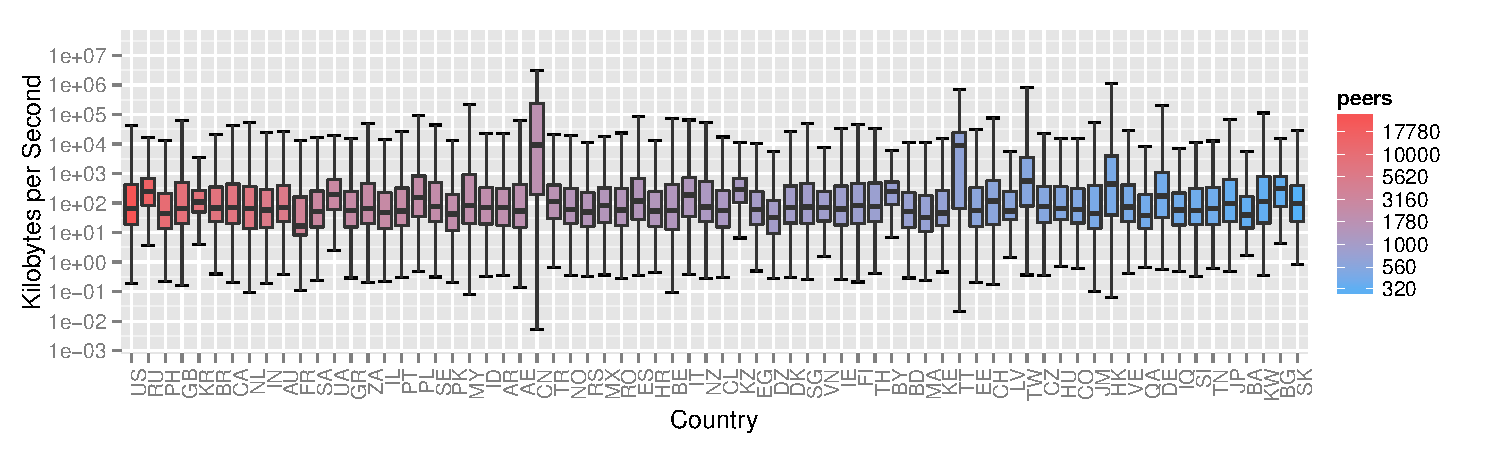
\includegraphics[width=\textwidth]{../result/2015-08-30_20-combined_speed_plot}
\caption[Download speed per country as box plot]{Download speeds of the \numprint{70} countries with most recorded unique peers, using a logarithmic scale for speeds and peer count. This graph uses a standard box plot with first and third quartiles as box delimiters and the median inside the box. Countries are sorted descending for the number of observed peers. \numprint{179} other country codes are not represented in this chart.}
\label{speed-boxes}
\end{figure}

\begin{figure}
\centering
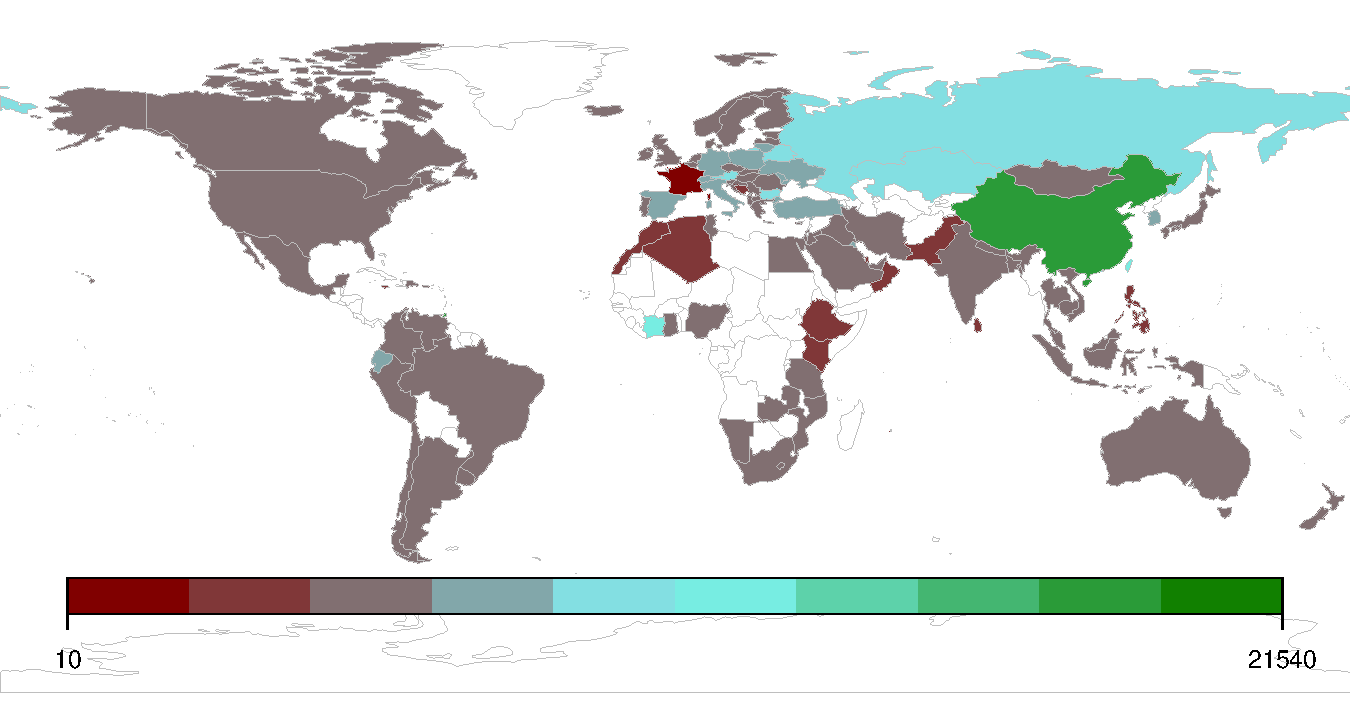
\includegraphics[width=\textwidth]{../result/2015-08-30_20-combined_speed_map}
\caption[Download speed per country as map]{Download speed per country as a map. Only countries with a minimum of about \numprint{50} observed peers are shown. Speed is given in kB/s on an logarithmic color scale. \numprint{149} other country codes are not represented in this map.}
\label{speed-map}
\end{figure}

When the download progress of a peer changes between two visits, a speed value can be calculated. This has been done for all peers during the analysis, while only keeping the maximum speed measured between too visits per peer. Figure \ref{speed-boxes} shows the results sorted by the number of unique peers. The median speed is mostly about \numprint[kB/s]{100}, while the majority of measurements are lying between \numprint[kB/s]{10} \numprint[MB/s]{1}. Standing out are China and Trinidad and Tobago with a median speed of nearly \numprint[MB/s]{10}. Most peers come from the United States, followed by Russia, the Philippines, the United Kingdom and South Korea. Speed values are drawn in a map in figure \ref{speed-map}.

\subsection{Internet Service Providers}
The data of hostnames was not extracted from the main analysis pass, but from an earlier one. Hostnames of peers were determined by performing a reverse DNS lookup on the IP address. This was performed by the storage module in the same thread which takes results from the \emph{visited queue} and writes them to the database. Since this lookup took about \numprint[ms]{300} on average, this is too slow for the database thread and was disabled during the main analysis run.
A solution to this problem, which is not implemented in the analysis tool, would be to perform the DNS lookups in a dedicated thread.

\begin{figure}
\centering
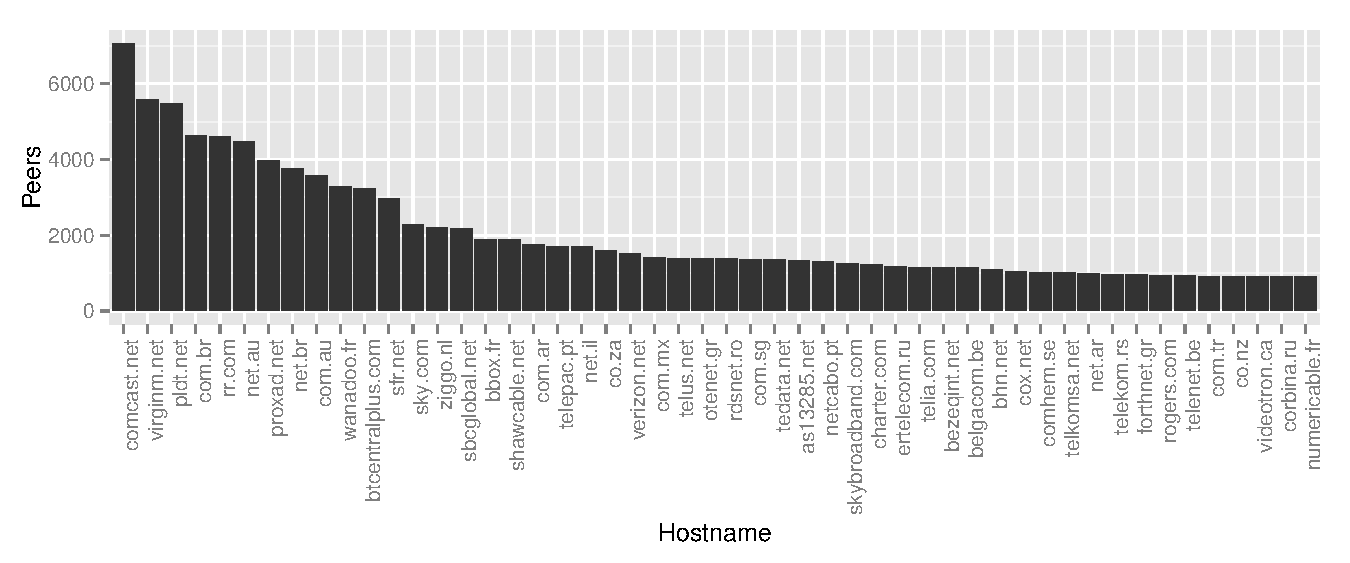
\includegraphics[width=\textwidth]{../result/2015-08-26_11-24-21_faui1-246_hostnames}
\caption[Most observed ISPs by hostname]{Top 50 hostnames of all unique observed peers. Only the TLD and SLD of hostnames were recorded. The majority of hostnames represent the used ISPs or seedbox providers, which are rentable servers optimized for usage with BitTorrent. Data is taken from a separate examination of twelve torrents which were chosen equivalently to the description of section \ref{cho}. Data is taken from the database \texttt{2015-08-26\_11-24-21\_faui1-246.sqlite}.}
\label{hostname}
\end{figure}

The data shown in figure \ref{hostname} used the peer contact and server threads to perform the reverse DNS lookups. However, this was not a reasonable fix for the problem, because as most peer contacts are revisits, this produces too many DNS requests for the university's DNS server. The most common hostnames among peers represent the following organizations:
\begin{enumerate}
\item ISP \textsc{Comcast} form the United States
\item ISP \textsc{Virgin Media} from the United Kingdom
\item ISP \textsc{Philippine Long Distance Telephone} from the Philippines
\item \texttt{com.br} is a second-level category for the Brazilian TLD
\item ISP \textsc{Time Warner Cable} from the United States, formerly known as \textsc{Road Runner}
\end{enumerate}
%%%%%%%%%%%%%%%%%%%%%%%%%%%%%%%%%%%%%%%%%%%%%%%%%%%%%%%%%%%%%%%%%%%%%%%%%%%%%%%%%

\chapter{Conclusion and Future Work}
\label{conc}
Existing problems of the BitTorrent Download Analyzer were discussed in section \ref{problems}. When encountering an error while evaluating a peer, the peer is excluded from further contacts. The evaluation of a newly collected peer address succeeded in \numprint[\%]{9} of cases. The success rate on the second visit was again only \numprint[\%]{15}, while the delay between two visits is five minutes. These values have to be increased in order to derive conclusive results. The fact that the success rate of a second evaluation for an incoming peers is as high as \numprint[\%]{78}, suggests the presence of a systematic problem.

A possible solution is to retry evaluation on failed peers after a longer delay. This could improve the chance of clients allowing a connection after receiving no data in the first session. Other helpful clues could be obtained by directly studying the behavior of common BitTorrent applications and make appropriate adjustments to the analyzer tool.

The requirement of two successful evaluations of a peer could be reduced to one, when running the analysis over a longer time. Uploading peers, who finished the download before the analysis was started would then be included in the result. However, after all seeding peers are registered, measured numbers should be comparable. This would reduce the complexity of the analysis method.
The process can be simplified even further by only sending ping requests to collected peer addresses to test their reachability, but this would defeat the goal of measuring confirmed downloads.

To increase the accuracy of comparison values for the number of downloads, scrape requests from all trackers should be included. The overlapping of peers between these trackers has to be compensated by considering the subset of peers which is known to each tracker. This can be done by requesting all peers through normal announce requests from all trackers.
%%%%%%%%%%%%%%%%%%%%%%%%%%%%%%%%%%%%%%%%%%%%%%%%%%%%%%%%%%%%%%%%%%%%%%%%%%%%%%%%%

\setcounter{biburllcpenalty}{7000}
\setcounter{biburlucpenalty}{8000}
\printbibheading[heading=bibintoc]
\begingroup
\setlength\labelnumberwidth{0.57cm}
\printbibliography[heading=subbibintoc, title={Literature}, keyword=science]
\printbibliography[heading=subbibintoc, title={Software}, keyword=software]
\printbibliography[heading=subbibintoc, title={Online}, keyword=online]
\printbibliography[heading=subbibintoc, title={Other}, notkeyword=science, notkeyword=standard, notkeyword=software, notkeyword=online] % TODO: remove, should be empty *
\endgroup
\printbibliography[heading=subbibintoc, title={Standards}, keyword=standard]
\end{document}
